% *******************************************************************
% STOP - Bitte zuerst lesen, bevor Sie weitermachen
%
% Einige Dinge müssen Sie an Ihre Bedürfnisse (und die Vorgaben Ihres
% Betreuers anpassen).
%
% 1. Sprache
% Das Template unterstützt Deutsch und Englisch, Standard ist Deutsch.
% Wenn Sie Englisch verwenden wollen, ändern Sie bitte direkt am Anfang
% dieser Datei den Eintrag
%    \newcommand{\hsmasprache}{de}
% auf
%    \newcommand{\hsmasprache}{en}
%
% 2. Form der Abgabe
% Das Template unterstützt sowohl eine digitale Abgabe, als auch eine Abgabe
% auf Papier. Bei einer Papierabgabe wird ein doppelseitiger Druck vorbereitet
% und der Titel wird so platziert, dass er in das Fenster des offiziellen
% Umschlages der Hochschule passt.
% Bei einer digitalen Abgabe (als PDF) wird der Titel zentriert und als
% Format wird einseitig gewählt. Außerdem wird die Datei unterschrift.png
% auf dem Blatt mit der Erklärung zur Eigenständigkeit eingebunden.
%
% 3. Zitierstil
% Abhängig von dem gewünschten Zitierstil passen Sie bitte in
% preambel.tex die Einstellungen bei \usepackage[backend=biber...
% an. Wie ist dort genau erklärt.
% Achtung: Wenn Sie als Zitierstil Fußnoten wählen bzw. generell
% -------  mit Fußnoten arbeiten, dann beachten Sie bitte, dass
%          Fußnoten in Bildunterschriften und Tabellenüberschriften
%          nicht funktionieren.
%          Siehe hierzu https://texfaq.org/FAQ-ftncapt
%          und https://texfaq.org/FAQ-footintab
%          Sinnvollerweise verzichten Sie auf Fußnoten an diesen
%          Stellen und fügen Quellen einfach per \parancite ein.
%
% 4. Doppelseitiger oder einseitiger Druck
% Das Template bestimmt, ob einseitig oder doppelseitig gedruckt wird
% anhand der Abgabeform (papier / digital). Wollen sie dies übersteuern,
% müssen Sie in der Datei preambel.tex folgende Zeile
% \KOMAoptions{twoside=true} für doppelsetigen Druck
% \KOMAoptions{twoside=false} für einsetigen Druck
% direkt vor \usepackage{xcolor} einsetzen. Prinzipiell sollten Sie aber
% das vorgeschlagene Format einfach so lassen.
%
% 5. Unnötige Teile entfernen
% Entfernen Sie die Teile, die Sie nicht brauchen, z.B. Anhänge,
% Quelltextverzeichnis etc. Siehe unten
%
% 6. Silbentrennung
% LaTeX führt eine automatische Silbentrennung durch. Allerdings
% werden Wörter, die bereits einen Bindestrich enthalten nicht
% getrennt, z.B. Datenschutz-Grundverordnung. Wenn Sie Ihren Text auf
% Deutsch schreiben, können Sie dann alternativ "= für den Bindestrich
% im Wort verwenden, z.B. Datenschutz"=Grundverordnung, damit LaTeX
% weiterhin richtig trennt.
% Ist die Silbentrennung aus einem anderen Grund nicht erfolgt, sodass
% das Wort über den rechten Rand hinaussteht oder wenn Sie eine weitere
% Trennstelle wollen, können Sie LaTeX helfen, indem Sie weitere
% Trennstellen angeben. Dies geschieht durch "- als Zeichen, z.B.
% Staats"-vertrag.
%
% 7. Nummerierung der Fußnoten
% LaTeX beginnt die Nummerierung der Fußnoten in jedem Kapitel wieder
% bei 1. Manche Dozenten wollen aber eine durchlaufende Nummerierung
% über die gesamte Arbeit. In diesem Fall gehen Sie in die preambel.tex
% und kommentieren den Befehl \counterwithout{footnote}{chapter} ein.
%
% 8. Unterschrift
% Bei einer Abgabe auf Papier unterschreiben Sie die Arbeit eigenhändig.
% Geben Sie allerdings digital ab, sollten Sie die Datei unterschrift.png
% durch einen Scan Ihrer eigenen Unteschrift ersetzen - andernfalls
% unterschreiben Sie als Max Mustermann ;-)
% *******************************************************************

% Sprache für das Dokument festlegen
\newcommand{\hsmasprache}{en}     % de oder en für Deutsch oder Englisch

% Abgabeform festlegen
% Bei einer digitalen Abgabe, wird das Dokument einseitig erzeugt und der Titel wird
% zentriert.
\newcommand{\hsmaabgabe}{digital} % Wie erfolgt die Abgabe: "papier" oder "digital"?

% Preambel mit Einstellungen importieren
% Pakete einbinden, die benötigt werden
\usepackage{scrpage2}
\usepackage{graphicx}             % Bilder einbinden
\usepackage{xcolor}               % Color support
\usepackage{amsmath}              % Matheamtische Formeln
\usepackage{amsfonts}             % Mathematische Zeichensätze
\usepackage{amssymb}              % Mathematische Symbole
\usepackage{float}                % Fließende Objekte (Tabellen, Grafiken etc.)
\usepackage{booktabs}             % Korrekter Tabellensatz
\usepackage[printonlyused]{acronym}  % Abkürzungsverzeichnis [nur verwendete Abkürzugen]
\usepackage{makeidx}              % Sachregister
\usepackage{listings}             % Source Code listings
\usepackage{listingsutf8}         % Listings in UTF8
\usepackage[hang,font={sf,footnotesize},labelfont={footnotesize,bf}]{caption} % Beschriftungen
\usepackage[scaled]{helvet}       % Schrift Helvetia laden
\usepackage[sf,bf,small]{titlesec} % Einstellungen für Überschriften
\usepackage[absolute]{textpos}	  % Absolute Textpositionen (für Deckblatt)
\usepackage{calc}                 % Berechnung von Positionen
\usepackage{blindtext}            % Blindtexte
\usepackage[bottom=40mm,left=35mm,right=35mm,top=30mm]{geometry} % Ränder ändern
\usepackage{setspace}             % Abstände korrigieren
\usepackage{ifthen}               % Logische Bedingungen mit ifthenelse
\usepackage{scrhack}              % Get rid of tocbasic warnings
\usepackage{lastpage}			  % Anzahl Seiten; für Titelblattt
%\usepackage[pagebackref=false]{hyperref}  % Hyperlinks
%\usepackage{rotating}             % Seiten drehen

%\setlength{\bibitemsep}{1em}     % Abstand zwischen den Literaturangaben
%\setlength{\bibhang}{2em}        % Einzug nach jeweils erster Zeile

% Farben definieren
\definecolor{linkblue}{RGB}{0, 0, 100}
\definecolor{linkblack}{RGB}{0, 0, 0}
\definecolor{comment}{RGB}{63, 127, 95}
\definecolor{darkgreen}{RGB}{14, 144, 102}
\definecolor{darkblue}{RGB}{0,0,168}
\definecolor{darkred}{RGB}{128,0,0}
\definecolor{javadoccomment}{RGB}{0,0,240}

% Einstellungen für das Hyperlink-Paket
\hypersetup{
    colorlinks=true,      % Farbige links verwenden       
%    allcolors=linkblue,
    linktoc=all,          % Links im Inhaltsverzeichnis
    linkcolor=linkblack,  % Querverweise
    citecolor=linkblack,  % Literaturangaben
	filecolor=linkblack,  % Dateilinks
	urlcolor=linkblack    % URLs
}

% Einstellungen für Quelltexte
\lstset{     
      xleftmargin=0.2cm,     
      basicstyle=\footnotesize\ttfamily,
      keywordstyle=\color{darkgreen},
      identifierstyle=\color{darkblue},
      commentstyle=\color{comment}, 
      stringstyle=\color{darkred}, 
      tabsize=2,
      lineskip={2pt},
      columns=flexible,
      inputencoding=utf8,
      captionpos=b,
      breakautoindent=true,
	  breakindent=2em,
	  breaklines=true,
	  prebreak=,
	  postbreak=,
      numbers=none,
      numberstyle=\tiny,
      showspaces=false,      % Keine Leerzeichensymbole
      showtabs=false,        % Keine Tabsymbole
      showstringspaces=false,% Leerzeichen in Strings
      morecomment=[s][\color{javadoccomment}]{/**}{*/},
      literate={Ö}{{\"O}}1 {Ä}{{\"A}}1 {Ü}{{\"U}}1 {ß}{{\ss}}2 {ü}{{\"u}}1 {ä}{{\"a}}1 {ö}{{\"o}}1
}

\urlstyle{same}

\titlespacing{\paragraph}{0pt}{1ex}{2.0ex}
\titlespacing{\subsubsection}{0pt}{3ex}{0.0ex}
\titlespacing{\subsection}{0pt}{4ex}{0.2ex}
\titlespacing{\section}{0pt}{7ex}{1ex}
\titleformat*{\subsubsection}{\sffamily\itshape\bfseries\small}
\titleformat*{\paragraph}{\sffamily\bfseries\small}


% Einstellungen für Überschriften
\renewcommand*{\chapterformat}{%
  \Large\chapapp~\thechapter   % Große Schrift
  \vspace{0.3cm}               % Abstand zum Titel des Kapitels
}

% Abstände für die Überschriften setzen

% In der Kopfzeile nur die kurze Kapitelbezeichnung (ohne Kapitel davor)
\renewcommand*\chaptermarkformat{\thechapter\autodot\enskip}
\automark[chapter]{chapter}

% Einstellungen für Schriftarten
\setkomafont{pagehead}{\normalfont\sffamily}
\setkomafont{pagenumber}{\normalfont\sffamily}
\setkomafont{paragraph}{\sffamily\bfseries\small}
\setkomafont{subsubsection}{\sffamily\itshape\bfseries\small}
\addtokomafont{footnote}{\footnotesize}
\setkomafont{chapter}{\LARGE\selectfont\bfseries}

% Wichtige Abstände
\setlength{\parskip}{0.2cm}  % 2mm Abstand zwischen zwei Absätzen
\setlength{\parindent}{0mm}  % Absätze nicht einziehen
\clubpenalty = 10000         % Keine "Schusterjungen"
\widowpenalty = 10000        % Keine "Hurenkinder"
\displaywidowpenalty = 10000 % Keine "Hurenkinder"
\renewcommand{\footnotesize}{\fontsize{9}{10}\selectfont} % Größe der Fußnoten
\setlength{\footnotesep}{8pt} % Abstand zwischen den Fußnoten

% Index erzeugen
\makeindex

% Einfacher Font-Wechsel über dieses Makro
\newcommand{\changefont}[3]{
\fontfamily{#1} \fontseries{#2} \fontshape{#3} \selectfont}

% Eigenes Makro für Bilder
\newcommand{\bild}[3]{
\begin{figure}[h]
  \centering
  \includegraphics[width=#2]{#1}
  \caption{#3}
  \label{#1}
\end{figure}}

% Wo liegt Sourcecode?
\newcommand{\srcloc}{src/}

% Wo sind die Bilder?
\graphicspath{{bilder/}}

% Makros für typographisch korrekte Abkürzungen
\newcommand{\zb}[0]{z.\,B.\ }
\newcommand{\dahe}[0]{d.\,h.\ }
\newcommand{\ua}[0]{u.\,a.\ }

% Flags für Veröffentlichung und Sperrvermerk
\newboolean{hsmapublizieren}
\newboolean{hsmasperrvermerk}


% Dokumenteninfos importieren
% -------------------------------------------------------
% Daten für die Arbeit
% Wenn hier alles korrekt eingetragen wurde, wird das Titelblatt
% automatisch generiert. D.h. die Datei titelblatt.tex muss nicht mehr
% angepasst werden.

% Titel der Arbeit auf Deutsch
\newcommand{\hsmatitelde}{Anforderungsdokument für ein Telemetriedatenvisualiserungsdashboard für die Caruso GmbH}

% Titel der Arbeit auf Englisch
\newcommand{\hsmatitelen}{Requirements Specification for a telemetry data visualization dashboard for Caruso GmbH}

% Weitere Informationen zur Arbeit
\newcommand{\hsmaort}{Mannheim}          % Ort
\newcommand{\hsmaautorvname}{Jan Diekhoff, Marvin Karhan, Jan Mayer, Joel Staubach}
\newcommand{\hsmaautorcontact}{eighteyes.info@gmail.com} % Kontaktadresse
\newcommand{\hsmaautornname}{} % Nachname(n)
\newcommand{\hsmadatum}{06.12.2022}      % Datum der Abgabe
\newcommand{\hsmajahr}{2022}             % Jahr der Abgabe
\newcommand{\hsmafirma}{Caruso GmbH} % Firma bei der die Arbeit durchgeführt wurde
\newcommand{\hsmabetreuer}{Prof. Dr. Peter Knauber, Hochschule Mannheim} % Betreuer an der Hochschule
\newcommand{\hsmazweitkorrektor}{Prof. Kirstin Kohler, Hochschule Mannheim}   % Betreuer im Unternehmen oder Zweitkorrektor
\newcommand{\hsmafakultaet}{I}    % I für Informatik oder E, S, B, D, M, N, W, V
\newcommand{\hsmastudiengang}{IB} % IB IMB UIB CSB IM MTB (weitere siehe titleblatt.tex)
\newcommand{\hsmaversion}{0.14} % Version

% Zustimmung zur Veröffentlichung
\setboolean{hsmapublizieren}{true}   % Einer Veröffentlichung wird zugestimmt
\setboolean{hsmasperrvermerk}{false} % Die Arbeit hat keinen Sperrvermerk

% "Creative Commons"-Lizenzen (https://creativecommons.org/)
% wenn Zustimmung zur Veröffentlichung und kein Sperrvermerk
%\renewcommand{\hsmacc}{by}
\renewcommand{\hsmacc}{by-sa}
%\renewcommand{\hsmacc}{by-nc-sa}

% -------------------------------------------------------
% Abstract
% Achtung: Wenn Sie im Abstrakt Anführungszeichen verwenden wollen, dann benutzen Sie
%          nicht "` und "', sondern \enquote{}. "` und "' werden nicht richtig
%          erkannt.



\usepackage[type={CC},modifier={\hsmacc},version={4.0}]{doclicense}
% Richtige Titel für das Quellcodeverzeichnis
\renewcommand\lstlistingname{\hsmalistingcaption}
\renewcommand\lstlistlistingname{\hsmalistings}

% Literatur-Datenbank
\addbibresource{literatur.bib}   % BibLaTeX-Datei mit Literaturquellen einbinden

% Anfang des Dokuments
\begin{document}

%Laden der Abkürzungen, Glossar, Symbole
% Tragen Sie hier alle Abkürzungen ein, die in der Arbeit benutzt werden
\newacronym{abk}{ABK}{Abkürzung}
\newacronym{acm}{ACM}{Association of Computing Machinery}
\newacronym{pdf}{PDF}{Portable Document Format}
\newacronym{ieee}{IEEE}{Institute of Electrical and Electronics Engineers}
\newacronym{iso}{ISO}{International Organization for Standardization}
\newacronym[plural=ISPs,firstplural=Internet Service Providers (ISPs)]{isp}{ISP}{Internet Service Provider}

% Glossareinträge
% \newglossaryentry{amplification}{name={Amplification}, description={describes the disproportionate increase of a response packet compared to the initial request packet.}}
\newglossaryentry{api}{name={Caruso API}, description={The Caruso interface through which vehicle data is received from the OEMs and vehicles can be registered.}}
\newglossaryentry{dataplace}{name={Caruso dataplace}, description={A digital marketplace where Caruso sells subscriptions to data items.}}
\newglossaryentry{subscription}{name={Caruso dataplace subscription}, description={A subscription to one or more data items in the Caruso dataplace.}}
\newglossaryentry{ci}{name={CI}, description={Corporate identity. The manner in which a company presents itself and its products to the public, for example logos, colours or brands.}}
\newglossaryentry{appetiser}{name={data appetiser}, description={A presentation showcasing Caruso data items.}}
\newglossaryentry{data}{name={data item}, description={A single standardised point of data sold in the Caruso dataplace.}}
\newglossaryentry{moscow}{name={MoSCoW method}, description={A prioritisation method for requirements. Stands for Must have, Should have Could have and Won't have.}}
\newglossaryentry{nontechnical}{name={non-technical}, description={A person who uses or otherwise interacts with Caruso data items without deeper knowledge or understanding of the technology behind them.}}
\newglossaryentry{oem}{name={OEM}, description={Original equipment manufacturer. The car manufacturers who sell the raw vehicle data to Caruso.}}
\newglossaryentry{persona}{name={persona}, description={A fictional person representative of a stakeholder in the project.}}
\newglossaryentry{stakeholder}{name={stakeholder}, description={A person, group, company or other entity who is impacted by the success of the project. Can be seperated into the core target group, direct stakeholders and indirect stakeholders.}}
\newglossaryentry{telemetry}{name={telematics data}, description={Data that is automatically gathered and transmitted during the use of a vehicle such as position, fuel gauge or indicator lamps.}}
\newglossaryentry{usecase}{name={use case}, description={A standalone action the user wants to take with the help of the application to achieve a specific goal.}}
\newglossaryentry{userstory}{name={user story}, description={A requirement in the form \enquote{as a \emph{role} I want to \emph{action} to achieve \emph{goal}}}, plural={user stories}}
\newglossaryentry{vin}{name={VIN}, description={Vehicle identification number. A unique identifier for a vehicle. Used to register vehicles in the Caruso dataplace. Used by both technical and non-technical people.}}
\newglossaryentry{widget}{name={widget}, description={A small, standalone piece of the user interface built for a single purpose.}}
% Verzeichnis von Symbolen und Einheiten
\newglossaryentry{symb:Pi}{name=\ensuremath{\pi},
	description={Geometrical value},
	unit={},
	type=symbolslist}

\newglossaryentry{symb:energyconsump}{name=\ensuremath{P},
	description={Energy consumption},
	unit={\si{kW}},
	type=symbolslist}


\frontmatter

% Römische Ziffern für die "Front-Matter"
\setcounter{page}{0}
\changefont{ptm}{m}{n}  % Times New Roman für den Fließtext
\renewcommand{\rmdefault}{ptm}

% Titelblatt
% *******************************************************************
% In dieser Datei sollten eigentlich keine Veränderungen
% notwendig sein. Alle Einstellungen erfolgen in docinfo.tex und
% der thesis.tex.
% *******************************************************************

\thispagestyle{empty}

% Fakultäten der HS-Mannheim
% *******************************************************************
\ifthenelse{\equal{\hsmafakultaet}{I}}%
  {\newcommand{\hsmafakultaetlangde}{Fakultät für Informatik}%
   \newcommand{\hsmafakultaetlangen}{Department of Computer Science}}{}

\ifthenelse{\equal{\hsmafakultaet}{E}}%
  {\newcommand{\hsmafakultaetlangde}{Fakultät für Elektrotechnik}%
   \newcommand{\hsmafakultaetlangen}{Department of Electrical Engineering}}{}

\ifthenelse{\equal{\hsmafakultaet}{S}}%
  {\newcommand{\hsmafakultaetlangde}{Fakultät für Sozialwesen}%
   \newcommand{\hsmafakultaetlangen}{Department of Social Work}}{}

\ifthenelse{\equal{\hsmafakultaet}{B}}%
  {\newcommand{\hsmafakultaetlangde}{Fakultät für Biotechnologie}%
   \newcommand{\hsmafakultaetlangen}{Department of Biotechnology}}{}

\ifthenelse{\equal{\hsmafakultaet}{D}}%
  {\newcommand{\hsmafakultaetlangde}{Fakultät für Gestaltung}%
   \newcommand{\hsmafakultaetlangen}{Department of Design}}{}

\ifthenelse{\equal{\hsmafakultaet}{M}}%
  {\newcommand{\hsmafakultaetlangde}{Fakultät für Maschinenbau}%
   \newcommand{\hsmafakultaetlangen}{Department of Mechanical Engineering}}{}

\ifthenelse{\equal{\hsmafakultaet}{N}}%
  {\newcommand{\hsmafakultaetlangde}{Fakultät für Informationstechnik}%
   \newcommand{\hsmafakultaetlangen}{Department of Information Technology}}{}

\ifthenelse{\equal{\hsmafakultaet}{W}}%
  {\newcommand{\hsmafakultaetlangde}{Fakultät für Wirtschaftsingenieurwesen}%
   \newcommand{\hsmafakultaetlangen}{Department of Engineering and Management}}{}

\ifthenelse{\equal{\hsmafakultaet}{V}}%
  {\newcommand{\hsmafakultaetlangde}{Fakultät für Verfahrens- und Chemietechnik}%
   \newcommand{\hsmafakultaetlangen}{Department of Chemical Process Engineering}}{}

% Studiengänge der HS-Mannheim
% *******************************************************************
\ifthenelse{\equal{\hsmastudiengang}{IB}}%
  {\newcommand{\hsmastudienganglangde}{Informatik}%
  \newcommand{\hsmastudienganglangen}{Computer Science}%
  \newcommand{\hsmatypde}{Bachelor-Thesis}%
  \newcommand{\hsmatypen}{Bachelor Thesis}%
  \newcommand{\hsmagrad}{\hsmabsc}}{}

\ifthenelse{\equal{\hsmastudiengang}{IMB}}%
  {\newcommand{\hsmastudienganglangde}{Medizinische Informatik}%
  \newcommand{\hsmastudienganglangen}{Medical Informatics}%
  \newcommand{\hsmatypde}{Bachelor-Thesis}%
  \newcommand{\hsmatypen}{Bachelor Thesis}%
  \newcommand{\hsmagrad}{\hsmabsc}}{}

\ifthenelse{\equal{\hsmastudiengang}{UIB}}%
  {\newcommand{\hsmastudienganglangde}{Unternehmens- und Wirtschaftsinformatik}%
  \newcommand{\hsmastudienganglangen}{Enterprise Computing}%
  \newcommand{\hsmatypde}{Bachelor-Thesis}%
  \newcommand{\hsmatypen}{Bachelor Thesis}%
  \newcommand{\hsmagrad}{\hsmabsc}}{}

\ifthenelse{\equal{\hsmastudiengang}{CSB}}%
  {\newcommand{\hsmastudienganglangde}{Cyber Security}%
  \newcommand{\hsmastudienganglangen}{Cyber Security}%
  \newcommand{\hsmatypde}{Bachelor-Thesis}%
  \newcommand{\hsmatypen}{Bachelor Thesis}%
  \newcommand{\hsmagrad}{\hsmabsc}}{}

\ifthenelse{\equal{\hsmastudiengang}{IM}}%
  {\newcommand{\hsmastudienganglangde}{Informatik}%
   \newcommand{\hsmastudienganglangen}{Computer Science}%
   \newcommand{\hsmatypde}{Master-Thesis}%
   \newcommand{\hsmatypen}{Master Thesis}%
   \newcommand{\hsmagrad}{\hsmamaster}}{}

\ifthenelse{\equal{\hsmastudiengang}{MEB}}%
  {\newcommand{\hsmastudienganglangde}{Mechatronik}%
   \newcommand{\hsmastudienganglangen}{Mechatronic}%
   \newcommand{\hsmatypde}{Bachelor-Thesis}%
   \newcommand{\hsmatypen}{Bachelor Thesis}%
   \newcommand{\hsmagrad}{\hsmabsc}}{}

\ifthenelse{\equal{\hsmastudiengang}{UB}}%
  {\newcommand{\hsmastudienganglangde}{Automatisierungstechnik}%
   \newcommand{\hsmastudienganglangen}{Automation Technology}%
   \newcommand{\hsmatypde}{Bachelor-Thesis}%
   \newcommand{\hsmatypen}{Bachelor Thesis}%
   \newcommand{\hsmagrad}{\hsmabsc}}{}

\ifthenelse{\equal{\hsmastudiengang}{ELB}}%
  {\newcommand{\hsmastudienganglangde}{Elektro- und Informationstechnik/Ingenieurpädagogik}%
   \newcommand{\hsmastudienganglangen}{Elektro- und Informationstechnik/Ingenieurpädagogik}%
   \newcommand{\hsmatypde}{Bachelor-Thesis}%
   \newcommand{\hsmatypen}{Bachelor Thesis}%
   \newcommand{\hsmagrad}{\hsmabsc}}{}

\ifthenelse{\equal{\hsmastudiengang}{EBE}}%
  {\newcommand{\hsmastudienganglangde}{Energietechnik und erneuerbare Energien}%
   \newcommand{\hsmastudienganglangen}{Power Engineering ans Renewable Energies}%
   \newcommand{\hsmatypde}{Bachelor-Thesis}%
   \newcommand{\hsmatypen}{Bachelor Thesis}%
   \newcommand{\hsmagrad}{\hsmabsc}}{}

\ifthenelse{\equal{\hsmastudiengang}{TS}}%
  {\newcommand{\hsmastudienganglangde}{Translation Studies}%
   \newcommand{\hsmastudienganglangen}{Translation Studies}%
   \newcommand{\hsmatypde}{Bachelor-Thesis}%
   \newcommand{\hsmatypen}{Bachelor Thesis}%
   \newcommand{\hsmagrad}{\hsmabsc}}{}

\ifthenelse{\equal{\hsmastudiengang}{EM}}%
  {\newcommand{\hsmastudienganglangde}{Automatisierungs- und Energiesysteme}%
   \newcommand{\hsmastudienganglangen}{Automation and Energy Systems}%
   \newcommand{\hsmatypde}{Master-Thesis}%
   \newcommand{\hsmatypen}{Master Thesis}%
   \newcommand{\hsmagrad}{\hsmamaster}}{}

\ifthenelse{\equal{\hsmastudiengang}{ELM}}%
  {\newcommand{\hsmastudienganglangde}{Lehramt Ingenieurpädagogik}%
   \newcommand{\hsmastudienganglangen}{Lectureship Educational Engineering}%
   \newcommand{\hsmatypde}{Master-Thesis}%
   \newcommand{\hsmatypen}{Master Thesis}%
   \newcommand{\hsmagrad}{\hsmamaster}}{}

\ifthenelse{\equal{\hsmastudiengang}{SAB}}%
  {\newcommand{\hsmastudienganglangde}{Soziale Arbeit}%
   \newcommand{\hsmastudienganglangen}{Social Labour}%
   \newcommand{\hsmatypde}{Bachelor-Thesis}%
   \newcommand{\hsmatypen}{Bachelor Thesis}%
   \newcommand{\hsmagrad}{\hsmaba}}{}

\ifthenelse{\equal{\hsmastudiengang}{SAM}}%
  {\newcommand{\hsmastudienganglangde}{Soziale Arbeit}%
   \newcommand{\hsmastudienganglangen}{Social Labour}%
   \newcommand{\hsmatypde}{Master-Thesis}%
   \newcommand{\hsmatypen}{Master Thesis}%
   \newcommand{\hsmagrad}{\hsmamastera}}{}

\ifthenelse{\equal{\hsmastudiengang}{BB}}%
  {\newcommand{\hsmastudienganglangde}{Biotechnology}%
   \newcommand{\hsmastudienganglangen}{Biotechnology}%
   \newcommand{\hsmatypde}{Bachelor-Thesis}%
   \newcommand{\hsmatypen}{Bachelor Thesis}%
   \newcommand{\hsmagrad}{\hsmabsc}}{}

\ifthenelse{\equal{\hsmastudiengang}{BCB}}%
  {\newcommand{\hsmastudienganglangde}{Biologische Chemie}%
   \newcommand{\hsmastudienganglangen}{Biological Chemics}%
   \newcommand{\hsmatypde}{Bachelor-Thesis}%
   \newcommand{\hsmatypen}{Bachelor Thesis}%
   \newcommand{\hsmagrad}{\hsmabsc}}{}

\ifthenelse{\equal{\hsmastudiengang}{BMEBST}}%
  {\newcommand{\hsmastudienganglangde}{Biotechnology - Biomedical Science and Technology}%
   \newcommand{\hsmastudienganglangen}{Biotechnology - Biomedical Science and Technology}%
   \newcommand{\hsmatypde}{Master-Thesis}%
   \newcommand{\hsmatypen}{Master Thesis}%
   \newcommand{\hsmagrad}{\hsmamaster}}{}

\ifthenelse{\equal{\hsmastudiengang}{BMEBPD}}%
  {\newcommand{\hsmastudienganglangde}{Biotechnology - Bioprocess Development}%
   \newcommand{\hsmastudienganglangen}{Biotechnology - Bioprocess Development}%
   \newcommand{\hsmatypde}{Master-Thesis}%
   \newcommand{\hsmatypen}{Master Thesis}%
   \newcommand{\hsmagrad}{\hsmamaster}}{}

\ifthenelse{\equal{\hsmastudiengang}{BLSM}}%
  {\newcommand{\hsmastudienganglangde}{Life Science Management}%
   \newcommand{\hsmastudienganglangen}{Life Science Management}%
   \newcommand{\hsmatypde}{Master-Thesis}%
   \newcommand{\hsmatypen}{Master Thesis}%
   \newcommand{\hsmagrad}{\hsmamaster}}{}

\ifthenelse{\equal{\hsmastudiengang}{KDB}}%
  {\newcommand{\hsmastudienganglangde}{Kommunikationsdesign}%
   \newcommand{\hsmastudienganglangen}{Communication Design}%
   \newcommand{\hsmatypde}{Bachelor-Thesis}%
   \newcommand{\hsmatypen}{Bachelor Thesis}%
   \newcommand{\hsmagrad}{\hsmaba}}{}

\ifthenelse{\equal{\hsmastudiengang}{KDM}}%
  {\newcommand{\hsmastudienganglangde}{Kommunikationsdesign}%
   \newcommand{\hsmastudienganglangen}{Communication Design}%
   \newcommand{\hsmatypde}{Master-Thesis}%
   \newcommand{\hsmatypen}{Master Thesis}%
   \newcommand{\hsmagrad}{\hsmamastera}}{}

\ifthenelse{\equal{\hsmastudiengang}{MB}}%
  {\newcommand{\hsmastudienganglangde}{Maschinenbau}%
   \newcommand{\hsmastudienganglangen}{Mechanical Engineering}%
   \newcommand{\hsmatypde}{Bachelor-Thesis}%
   \newcommand{\hsmatypen}{Bachelor Thesis}%
   \newcommand{\hsmagrad}{\hsmabsc}}{}

\ifthenelse{\equal{\hsmastudiengang}{MM}}%
  {\newcommand{\hsmastudienganglangde}{Maschinenbau}%
   \newcommand{\hsmastudienganglangen}{Mechanical Engineering}%
   \newcommand{\hsmatypde}{Master-Thesis}%
   \newcommand{\hsmatypen}{Master Thesis}%
   \newcommand{\hsmagrad}{\hsmamaster}}{}

\ifthenelse{\equal{\hsmastudiengang}{NEB}}%
  {\newcommand{\hsmastudienganglangde}{Elektronik}%
   \newcommand{\hsmastudienganglangen}{Electronics}%
   \newcommand{\hsmatypde}{Bachelor-Thesis}%
   \newcommand{\hsmatypen}{Bachelor Thesis}%
   \newcommand{\hsmagrad}{\hsmabsc}}{}

\ifthenelse{\equal{\hsmastudiengang}{TIB}}%
  {\newcommand{\hsmastudienganglangde}{Technische Informatik}%
   \newcommand{\hsmastudienganglangen}{Technical Information Technology}%
   \newcommand{\hsmatypde}{Bachelor-Thesis}%
   \newcommand{\hsmatypen}{Bachelor Thesis}%
   \newcommand{\hsmagrad}{\hsmabsc}}{}

\ifthenelse{\equal{\hsmastudiengang}{MTB}}%
  {\newcommand{\hsmastudienganglangde}{Medizintechnik}%
   \newcommand{\hsmastudienganglangen}{Medical Technology}%
   \newcommand{\hsmatypde}{Bachelor-Thesis}%
   \newcommand{\hsmatypen}{Bachelor Thesis}%
   \newcommand{\hsmagrad}{\hsmabsc}}{}

\ifthenelse{\equal{\hsmastudiengang}{MTM}}%
  {\newcommand{\hsmastudienganglangde}{Medizintechnik}%
   \newcommand{\hsmastudienganglangen}{Medical Technology}%
   \newcommand{\hsmatypde}{Master-Thesis}%
   \newcommand{\hsmatypen}{Master Thesis}%
   \newcommand{\hsmagrad}{\hsmamaster}}{}

\ifthenelse{\equal{\hsmastudiengang}{NM}}%
  {\newcommand{\hsmastudienganglangde}{Informationstechnik}%
   \newcommand{\hsmastudienganglangen}{Informationstechnik}%
   \newcommand{\hsmatypde}{Master-Thesis}%
   \newcommand{\hsmatypen}{Master Thesis}%
   \newcommand{\hsmagrad}{\hsmamaster}}{}

\ifthenelse{\equal{\hsmastudiengang}{WB}}%
  {\newcommand{\hsmastudienganglangde}{Wirtschaftsingenieurwesen}%
   \newcommand{\hsmastudienganglangen}{Engineering and Management}%
   \newcommand{\hsmatypde}{Bachelor-Thesis}%
   \newcommand{\hsmatypen}{Bachelor Thesis}%
   \newcommand{\hsmagrad}{\hsmabsc}}{}

\ifthenelse{\equal{\hsmastudiengang}{WM}}%
  {\newcommand{\hsmastudienganglangde}{Wirtschaftsingenieurwesen}%
   \newcommand{\hsmastudienganglangen}{Engineering and Management}%
   \newcommand{\hsmatypde}{Master-Thesis}%
   \newcommand{\hsmatypen}{Master Thesis}%
   \newcommand{\hsmagrad}{\hsmamaster}}{}

\ifthenelse{\equal{\hsmastudiengang}{WMI}}%
  {\newcommand{\hsmastudienganglangde}{Wirtschaftsingenieurwesen}%
   \newcommand{\hsmastudienganglangen}{Engineering and Management}%
   \newcommand{\hsmatypde}{Master-Thesis}%
   \newcommand{\hsmatypen}{Master Thesis}%
   \newcommand{\hsmagrad}{\hsmamaster}}{}

\ifthenelse{\equal{\hsmastudiengang}{WMB}}%
  {\newcommand{\hsmastudienganglangde}{Wirtschaftsingenieurwesen mit den\\ ingenieurwissenschaftlichen Fachrichtungen Maschinenbau und Elektrotechnik}%
   \newcommand{\hsmastudienganglangen}{Engineering and Management\\ with focus on Mechanical and Electrical Engineering}%
   \newcommand{\hsmatypde}{Master-Thesis}%
   \newcommand{\hsmatypen}{Master Thesis}%
   \newcommand{\hsmagrad}{\hsmamaster}}{}

\ifthenelse{\equal{\hsmastudiengang}{WMW}}%
  {\newcommand{\hsmastudienganglangde}{Wirtschaftsingenieurwesen mit\\ ingenieurwissenschaftlicher Vertiefung des Maschinenbaus}%
   \newcommand{\hsmastudienganglangen}{Engineering and Management\\ deepening the engineering aspects of Mechanical Engineering}%
   \newcommand{\hsmatypde}{Master-Thesis}%
   \newcommand{\hsmatypen}{Master Thesis}%
   \newcommand{\hsmagrad}{\hsmamaster}}{}

\ifthenelse{\equal{\hsmastudiengang}{VB}}%
  {\newcommand{\hsmastudienganglangde}{Verfahrenstechnik}%
   \newcommand{\hsmastudienganglangen}{Process Engineering}%
   \newcommand{\hsmatypde}{Bachelor-Thesis}%
   \newcommand{\hsmatypen}{Bachelor Thesis}%
   \newcommand{\hsmagrad}{\hsmabsc}}{}

\ifthenelse{\equal{\hsmastudiengang}{CB}}%
  {\newcommand{\hsmastudienganglangde}{Chemische Technik}%
   \newcommand{\hsmastudienganglangen}{Chemical Engineering}%
   \newcommand{\hsmatypde}{Bachelor-Thesis}%
   \newcommand{\hsmatypen}{Bachelor Thesis}%
   \newcommand{\hsmagrad}{\hsmabsc}}{}

\ifthenelse{\equal{\hsmastudiengang}{CM}}%
  {\newcommand{\hsmastudienganglangde}{Chemieingenieurwesen}%
   \newcommand{\hsmastudienganglangen}{Chemical Engineering}%
   \newcommand{\hsmatypde}{Master-Thesis}%
   \newcommand{\hsmatypen}{Master Thesis}%
   \newcommand{\hsmagrad}{\hsmamaster}}{}

% Abschlüsse
% *******************************************************************
\newcommand{\hsmabsc}{Bachelor of Science (B.Sc.)}
\newcommand{\hsmaba}{Bachelor of Arts (B.A.)}
\newcommand{\hsmamaster}{Master of Science (M.Sc.)}
\newcommand{\hsmamastera}{Master of Arts (M.A.)}
\newcommand{\hsmamasterba}{Master of Business Administration (MBA)}

\newcommand{\hsmakoerperschaftde}{Hochschule Mannheim}
\newcommand{\hsmakoerperschaften}{University of Applied Sciences Mannheim}

\newcommand{\hsmaautorbib}{\hsmaautornname \ \hsmaautorvname} % Autor Nachname, Vorname
\newcommand{\hsmaautor}{\hsmaautorvname \ \hsmaautornname} % Autor Vorname Nachname
\newcommand{\hsmacontact}{Contact us at: \hsmaautorcontact} % Autor Vorname Nachname

\ifthenelse{\equal{\hsmasprache}{de}}%
  {\newcommand{\hsmatyp}{\hsmatypde}%
   \newcommand{\hsmathesistype}{zur Erlangung des akademischen Grades \hsmagrad}%
   \newcommand{\hsmakoerperschaft}{\hsmakoerperschaftde}%
   \newcommand{\hsmastudiengangname}{Studiengang \hsmastudienganglangde}%
   \newcommand{\hsmastudienganglang}{\hsmastudienganglangde}%
   \newcommand{\hsmatitel}{\hsmatitelde}%
   \newcommand{\hsmatutor}{Betreuer}%
   \newcommand{\hsmafakultaetlang}{\hsmafakultaetlangde}%
   \newcommand{\hsmalistoftables}{Tabellenverzeichnis}%
   \newcommand{\hsmalistoffigures}{Abbildungsverzeichnis}%
   \newcommand{\hsmalistings}{Quellcodeverzeichnis}%
   \newcommand{\hsmalistofsymbols}{Symbolverzeichnis}
   \newcommand{\hsmaglossary}{Glossar}
   \newcommand{\hsmalistingcaption}{Listing}% oder Quellcode?
   \newcommand{\hsmasymbsign}{Symbol}
   \newcommand{\hsmasymbdescription}{Beschreibung}
   \newcommand{\hsmasymbunit}{Einheit}
   \newcommand{\hsmaindex}{Index}%
   \newcommand{\hsmaabbreviations}{Abkürzungsverzeichnis}%
   \newcommand{\hsmasnowcardanforderung}{Anforderung}%
   \newcommand{\hsmasnowcardno}{Nr}%
   \newcommand{\hsmasnowcardart}{Art}%
   \newcommand{\hsmasnowcardprio}{Prio}%
   \newcommand{\hsmasnowcardtitel}{Titel}%
   \newcommand{\hsmasnowcardherkunft}{Herkunft}%
   \newcommand{\hsmasnowcardkonflikt}{Konflikte}%
   \newcommand{\hsmasnowcardbeschreibung}{Beschreibung}%
   \newcommand{\hsmasnowcardfitkriterium}{Fit-Kriterium}%
   \newcommand{\hsmasnowcardmaterial}{Weiteres Material}%
   \newcommand{\hsmaqasanforderung}{QAS}%
   \newcommand{\hsmaqasno}{Nr}%
   \newcommand{\hsmaqasart}{Art}%
   \newcommand{\hsmaqasprio}{Priority}%
   \newcommand{\hsmaqastitel}{Titel}%
   \newcommand{\hsmaqasquelle}{Quelle}%
   \newcommand{\hsmaqasstimulus}{Stimulus}%
   \newcommand{\hsmaqasartefakt}{Artefakt}%
   \newcommand{\hsmaqasumgebung}{Umgebung}%
   \newcommand{\hsmaqasantwort}{Antwort}%
   \newcommand{\hsmaqasmass}{Maß für Antwort}%
   \newcommand{\hsmafirmatext}{In Kooperation mit der Firma }%
   \selectlanguage{ngerman}}%
  {\newcommand{\hsmatyp}{\hsmatypen}%
   \newcommand{\hsmathesistype}{for the acquisition of the academic degree \hsmagrad}%
   \newcommand{\hsmakoerperschaft}{\hsmakoerperschaften}%
   \newcommand{\hsmastudiengangname}{Course of Studies: \hsmastudienganglang}%
   \newcommand{\hsmastudienganglang}{\hsmastudienganglangen}%
   \newcommand{\hsmatitel}{\hsmatitelen}%
   \newcommand{\hsmatutor}{Tutors}
   \newcommand{\hsmafakultaetlang}{\hsmafakultaetlangen}%
   \newcommand{\hsmalistoftables}{List of Tables}%
   \newcommand{\hsmalistoffigures}{List of Figures}%
   \newcommand{\hsmalistings}{Listings}%
   \newcommand{\hsmalistingcaption}{Listing}% or Source Code?
   \newcommand{\hsmaindex}{Index}%
   \newcommand{\hsmasymbsign}{Sign}
   \newcommand{\hsmasymbdescription}{Description}
   \newcommand{\hsmasymbunit}{Unit}
   \newcommand{\hsmaabbreviations}{List of Abbreviations}%
   \newcommand{\hsmalistofsymbols}{List of Symbols}
   \newcommand{\hsmaglossary}{Glossary}
   \newcommand{\hsmasnowcardanforderung}{Requirement}%
   \newcommand{\hsmasnowcardno}{\#}%
   \newcommand{\hsmasnowcardart}{Type}%
   \newcommand{\hsmasnowcardprio}{Prio}%
   \newcommand{\hsmasnowcardtitel}{Title}%
   \newcommand{\hsmasnowcardherkunft}{Origin}%
   \newcommand{\hsmasnowcardkonflikt}{Conflicts}%
   \newcommand{\hsmasnowcardbeschreibung}{Description}%
   \newcommand{\hsmasnowcardfitkriterium}{Fit Criterion}%
   \newcommand{\hsmasnowcardmaterial}{Supporting Material}%
   \newcommand{\hsmaqasanforderung}{QAS}%
   \newcommand{\hsmaqasno}{\#}%
   \newcommand{\hsmaqasart}{Type}%
   \newcommand{\hsmaqasprio}{Prio}%
   \newcommand{\hsmaqastitel}{Title}%
   \newcommand{\hsmaqasquelle}{Source}%
   \newcommand{\hsmaqasstimulus}{Stimulus}%
   \newcommand{\hsmaqasartefakt}{Artifact}%
   \newcommand{\hsmaqasumgebung}{Environment}%
   \newcommand{\hsmaqasantwort}{Response}%
   \newcommand{\hsmaqasmass}{Response Measure}%
   \newcommand{\hsmafirmatext}{In cooperation with the company}%
   \selectlanguage{english}}%

% Daten in die Standard-Felder von KOMA-Script eintragen
\titlehead{\hsmatyp\ in\  \hsmastudienganglang}
\subject{}
\title{\hsmatitel}
\author{\hsmaauthor}
\date{\small{\hsmadatum}}

% Daten für das fertige PDF-Dokument
\hypersetup{
  pdftitle={\hsmatitel},                           % Titel des Dokuments
  pdfauthor={\hsmaautor},                          % Autor
  pdfsubject={\hsmatyp\ in\ \hsmastudienganglang}, % Thema
  pdfkeywords={\hsmatitel}                         % Schlüsselworte
}

\newlength{\bindekorrektur}
\newlength{\seitenanfang}
\newlength{\seitenbreite}

\setlength{\bindekorrektur}{-46mm}   % Korrektur der horizontalen Position
\setlength{\seitenanfang}{0mm}       % Korrektur der vertikalen Position
\setlength{\seitenbreite}{297mm}     % Breite der Seite

\noindent
\includegraphics[width=.45\columnwidth]{hsma-logo.pdf}\hfill
\noindent
\includegraphics[width=.45\columnwidth]{caruso_logo_rgb.png}\\

% Titel der Arbeit
\begin{textblock*}{128mm}(\hsmafenster,\seitenanfang + 62mm) % 4,5cm vom linken Rand und 6,0cm vom oberen Rand
  \centering\Large\sffamily
  \vspace{4mm} % Kleiner zusätzlicher Abstand oben für bessere Optik
  \textbf{\hsmatitel}
\end{textblock*}%


% Name
\begin{textblock*}{128mm}(\hsmafenster,\seitenanfang + 103mm)
  \centering\large\sffamily
  \hsmaautor\\
  \vspace{2mm}
  \hsmacontact
  
\includegraphics*[width=5cm]{./8eyes.png}
\end{textblock*}

% Thesis
% \begin{textblock*}{\seitenbreite}(\bindekorrektur,\seitenanfang + 130mm)
%   \centering\large\sffamily
  % \hsmatyp\\
  % \begin{small}\hsmathesistype \end{small}\\
%   \vspace{2mm}
% \end{textblock*}

% Fakultät
\begin{textblock*}{\seitenbreite}(\bindekorrektur,\seitenanfang + 165mm)
  \centering\large\sffamily
  \hsmastudiengangname\\
  \vspace{2mm}
  \hsmafakultaetlang\\
  \vspace{2mm}
  \hsmakoerperschaft
\end{textblock*}

% Datum
\begin{textblock*}{\seitenbreite}(\bindekorrektur,\seitenanfang + 205mm)
  \centering\large
  \textsf{\hsmadatum}\\
  \textsf{Version: \hsmaversion}
\end{textblock*}

% Firma
\begin{textblock*}{\seitenbreite}(\bindekorrektur,\seitenanfang + 225mm)
  \centering\large
  \textsf{\hsmafirmatext\,\hsmafirma}
\end{textblock*}

% Betreuer
\begin{textblock*}{\seitenbreite}(\bindekorrektur,\seitenanfang + 240mm)
  \centering\large\sffamily
  \hsmatutor \\
  \vspace{2mm}
  \hsmabetreuer\\
  \vspace{2mm}
  \hsmazweitkorrektor
\end{textblock*}

% Bibliographische Informationen
% \null\newpage
% \thispagestyle{empty}

% \newcommand{\hsmabibde}{\begin{small}\textbf{\hsmaautorbib}: \\ \hsmatitelde \ / \hsmaautor. \ -- \\ \hsmatypde, \hsmaort : \hsmakoerperschaftde, \hsmajahr. \pageref{lastpage} Seiten.\end{small}}

% \newcommand{\hsmabiben}{\begin{small}\textbf{\hsmaautorbib}: \\ \hsmatitelen \ / \hsmaautor. \ -- \\ \hsmatypen, \hsmaort : \hsmakoerperschaften, \hsmajahr. \pageref{lastpage} pages. \end{small}}

% % Reihenfolge hängt von der Sprache ab
% \ifthenelse{\equal{\hsmasprache}{de}}%
%   {\hsmabibde \\ \vspace{0.5cm} \\ \hsmabiben}
%   {\hsmabiben \\ \vspace{0.5cm} \\ \hsmabibde}

% Erklärung zur Eigenhändigkeit
% \clearpage\setcounter{page}{1}
% \thispagestyle{empty}
% \textsf{\large\textbf{Erklärung}}

% Hiermit erkläre ich, dass ich die vorliegende Arbeit selbstständig verfasst und keine anderen als die angegebenen Quellen und Hilfsmittel benutzt habe.

% \ifthenelse{\boolean{hsmapublizieren} \and \not\boolean{hsmasperrvermerk}}%
% {
% 	\ifthenelse{\equal{\hsmacc}{}}{
%   \vspace{0.5cm}
%   Ich bin damit einverstanden, dass meine Arbeit veröffentlicht wird, d.\,h. dass die Arbeit elektronisch gespeichert, in andere Formate konvertiert, auf den Servern der Hochschule Mannheim öffentlich zugänglich gemacht und über das Internet verbreitet werden darf.
%   }{\doclicenseThis}
% }{}%

% \vspace{1cm}
% \hsmaort, \hsmadatum \\

% \ifthenelse{\equal{\hsmaabgabe}{papier}}%
%   {%
%     % Papier - space
%     \vspace{1.2cm}
%   }%
%   {%
%     % Digital - Unterschrift
%     
\includegraphics[width=6cm]{unterschrift.png}
%   }%

% \hsmaautor

% Sperrvermerk
\ifthenelse{\boolean{hsmasperrvermerk}}%
{%
\vspace{11cm}
\color{red}\textsf{\large\textbf{Sperrvermerk}}

Diese Arbeit basiert auf internen und vertraulichen Daten des Unternehmens \hsmafirma.

Diese Arbeit darf Dritten, mit Ausnahme der betreuenden Dozenten und befugten Mitglieder des Prüfungsausschusses, ohne ausdrückliche Zustimmung des Unternehmens und des Verfassers nicht zugänglich gemacht werden.

Eine Vervielfältigung und Veröffentlichung der Arbeit ohne ausdrückliche Genehmigung -- auch in Auszügen -- ist nicht erlaubt.
\color{black}
}{}

\cleardoublepage

% Abstract
% \chapter*{Abstract}

% % Reihenfolge hängt von der Sprache ab
% \ifthenelse{\equal{\hsmasprache}{de}}%
% {
%   \subsubsection*{\hsmatitelde}
%   \hsmaabstractde
%   \begin{otherlanguage}{english}
%     \subsubsection*{\hsmatitelen}
%     \hsmaabstracten
%   \end{otherlanguage}
% }
% {
%   \subsubsection*{\hsmatitelen}
%   \hsmaabstracten
%   \begin{otherlanguage}{ngerman}
%     \subsubsection*{\hsmatitelde}
%     \hsmaabstractde
%   \end{otherlanguage}
% }

\newcounter{snowcardcounter}
\newcommand{\snowcard}[5]{
  \begin{table}[ht!]
    \stepcounter{snowcardcounter}
    \caption{\hsmasnowcardanforderung\ NFR\_{\arabic{snowcardcounter}} -- #3}\label{NFR{\arabic{snowcardcounter}}}
    \centering
    \sffamily
    \begin{footnotesize}
    \begin{tabularx}{\linewidth}{sssssb}
    \toprule
    \textbf{\hsmasnowcardno} & NFR\_{\arabic{snowcardcounter}} & \textbf{\hsmasnowcardart} & #1 & \textbf{\hsmasnowcardprio} & #2 \\
    \midrule
    \multicolumn{2}{l}{\textbf{\hsmasnowcardtitel}} & \multicolumn{4}{l}{\parbox[t]{11.8cm}{#3}} \\
    \addlinespace
    \multicolumn{6}{l}{\textbf{\hsmasnowcardbeschreibung}} \\
    \multicolumn{6}{l}{\parbox[t]{13.5cm}{#4}} \\
    \addlinespace
    \multicolumn{6}{l}{\textbf{\hsmasnowcardfitkriterium}} \\
    \multicolumn{6}{l}{\parbox{13.5cm}{#5}} \\
    \bottomrule
    \end{tabularx}
    \end{footnotesize}
  \end{table}
 }


% % Snowcard
%  \newcommand{\snowcard}[9]{
%    \begin{table}[ht!]
%  \caption{\hsmasnowcardanforderung\ #1 -- #4}\label{#1}
%  \renewcommand{\arraystretch}{1.2}
%  \centering
%  \sffamily
%    \begin{footnotesize}

%  \begin{tabularx}{\linewidth}{sssssb}
%  \toprule
%  \textbf{\hsmasnowcardno} & #1 & \textbf{\hsmasnowcardart} & #2 & \textbf{\hsmasnowcardprio} & #3 \\
%  \midrule
%  \multicolumn{2}{l}{\textbf{\hsmasnowcardtitel}} & \multicolumn{4}{l}{\parbox[t]{11.8cm}{#4}} \\
%  \ifx&#5&%
%  \else
%  \multicolumn{2}{l}{\textbf{\hsmasnowcardherkunft}} & \multicolumn{4}{l}{\parbox[t]{11.8cm}{#5}} \\
%  \fi
%  \ifx&#6&%
%  \else
%  \multicolumn{2}{l}{\textbf{\hsmasnowcardkonflikt}} & \multicolumn{4}{l}{\parbox[t]{11.8cm}{#6}} \\
%  \fi
%  \addlinespace
%  \multicolumn{6}{l}{\textbf{\hsmasnowcardbeschreibung}} \\
%  \multicolumn{6}{l}{\parbox[t]{13.5cm}{#7}} \\
%  \ifx&#8&%
%  \else
%  \addlinespace
%  \multicolumn{6}{l}{\textbf{\hsmasnowcardfitkriterium}} \\
%  \multicolumn{6}{l}{\parbox{13.5cm}{#8}} \\
%  \fi
%  \ifx&#9&%

%  \else
%    \addlinespace
%    \multicolumn{6}{l}{\textbf{\hsmasnowcardmaterial}} \\
%    \multicolumn{6}{l}{\parbox{13.5cm}{#9}} \\
%  \fi
%  \bottomrule
%  \end{tabularx}
%  \end{footnotesize}
%  \end{table}
% }

% % Quality Attribute Scenario
% \newcommand{\qas}[9]{
%   \begin{table}[ht!]
% \caption{\hsmaqasanforderung\ #1 -- #3}\label{#1}
% \renewcommand{\arraystretch}{1.2}
% \centering
% \sffamily
%   \begin{footnotesize}

% \begin{tabularx}{\linewidth}{sssssb}
% \toprule
% \textbf{\hsmaqasno} & #1 & \textbf{\hsmaqasart} & QAS & \textbf{\hsmaqasprio} & #2 \\
% \midrule
% \multicolumn{2}{l}{\textbf{\hsmaqastitel}} & \multicolumn{4}{l}{\parbox[t]{11.8cm}{#3}} \\
% \multicolumn{2}{l}{\textbf{\hsmaqasquelle}} & \multicolumn{4}{l}{\parbox[t]{11.8cm}{#4}} \\
% \multicolumn{2}{l}{\textbf{\hsmaqasstimulus}} & \multicolumn{4}{l}{\parbox[t]{11.8cm}{#5}} \\
% \multicolumn{2}{l}{\textbf{\hsmaqasartefakt}} & \multicolumn{4}{l}{\parbox[t]{11.8cm}{#6}} \\
% \addlinespace
% \multicolumn{6}{l}{\textbf{\hsmaqasumgebung}} \\
% \multicolumn{6}{l}{\parbox{13.5cm}{#7}} \\
% \addlinespace
% \multicolumn{6}{l}{\textbf{\hsmaqasantwort}} \\
% \multicolumn{6}{l}{\parbox{13.5cm}{#8}} \\
% \addlinespace
% \multicolumn{6}{l}{\textbf{\hsmaqasmass}} \\
% \multicolumn{6}{l}{\parbox{13.5cm}{#9}} \\
% \bottomrule
% \end{tabularx}
% \end{footnotesize}
% \end{table}
% }


\chapter{Change Log}
\definecolor{Gray}{gray}{0.8}

\sffamily
\begin{footnotesize}
  \renewcommand{\arraystretch}{1.4}
  \begin{longtable}[L L L L]{ p{.1\textwidth} p{.15\textwidth} p{.5\textwidth} p{.15\textwidth} }
    \caption                       % Caption für das Tabellenverzeichnis
    {Change log} % Caption für die Tabelle selbs
    \\
    \toprule
    \textbf{Version} & \textbf{Date} & \textbf{Description}                                                                                                                          & \textbf{Author} \\
    \midrule
    0.1              & 18.12.2022    & Setup of the intial document with table of contents                                                                                           & Marvin Karhan   \\

    \rowcolor{Gray}
    0.2              & 20.12.2022    & Add first key notes for the first chapter and modify the change log style                                                                     & Joel Staubach   \\

    0.3              & 21.12.2022    & Add non-functional requirement Chapters and outlook                                                                                           & Jan Mayer       \\

    \rowcolor{Gray}
    0.4              & 23.12.2022    & Add project background, goals and solution                                                                                                    & Joel Staubach   \\

    0.5              & 24.12.2022    & Add stakeholders chapter, except Personas                                                                                                     & Joel Staubach   \\

    \rowcolor{Gray}
    0.6              & 26.12.2022    & Add Current Situation, Context Of The Work, Product Boundary, Use Case Table, Individual Product Use Cases, Functional Requirements, Personas & Joel Staubach   \\

    0.7              & 30.12.2022    & Add Constraints and Relevant Facts and Assumptions                                                                                            & Marvin Karhan   \\

    \rowcolor{Gray}
    0.8              & 02.01.2023    & Add Security Requirements and Risks                                                                                                           & Marvin Karhan   \\

    0.9              & 04.01.2023    & Add chapter introduction Stakeholders, non-functional chapters                                                                                & Jan Mayer       \\

    \rowcolor{Gray}
    0.10             & 04.01.2023    & Add chapters Performance Requirements, Open Issues, Off the Shelf Solutions                                                                   & Jan Diekhoff    \\

    0.11             & 05.01.2023    & Translate German texts into English                                                                                                           & Jan Diekhoff    \\

    \rowcolor{Gray}
    0.12             & 05.01.2023    & Update chapters Scope of the Work, Scope of the Product and Functional Requirements                                                           & Jan Diekhoff    \\

    0.13             & 05.01.2023    & Update Remove the Open Issues chapter and incorporate it into Risks                                                                           & Marvin Karhan   \\

    \rowcolor{Gray}
    0.14             & 06.01.2023    & Added glossary                                                                                                                                & Jan Diekhoff    \\

    0.15             & 06.01.2023    & Update URLs and add smaller text passages                                                                                                     & Jan Mayer       \\
    
    \rowcolor{Gray}
    1.0              & 06.01.2023    & Prepare for peer review                                                                                                                       & All             \\
    
    1.1              & 18.01.2023    & Update Chapter 3, 4 and 5 based on feedback                                                                                                   & Marvin Karhan   \\

    \rowcolor{Gray}
    1.2              & 19.01.2023    & Various changes based on feedback, replacing of pictures with english variants, colouring tables                                              & Jan Diekhoff    \\
    
    1.3              & 20.01.2023    & Aggregated non-functional requirements into a single chapter with snow cards                                                                  & Jan Diekhoff, Jan Mayer    \\
    \bottomrule
  \end{longtable}
\end{footnotesize}
\rmfamily

% Inhaltsverzeichnis erzeugen
\cleardoublepage
\pdfbookmark{\contentsname}{Contents}
\tableofcontents
\cleardoublepage
\chapter{Introduction}
This document is intended to reflect the requirements of the \gls{appetiser} of the client Caruso GmbH. The purpose of the data appetiser is to demonstrate the value of \gls{telemetry} from cars to potential customers of Caruso.

The document is based on a scaled down version of the Requirements Specification Template Volere by James Robertson \& Suzanne Robertson and is intended to discuss the requirements for a solution to the required problem.
% Korrigiert Nummerierung bei mehrseitigem Inhaltsverzeichnis
\cleardoublepage
\newcounter{frontmatterpage}
\setcounter{frontmatterpage}{\value{page}}

% Arabische Zahlen für den Hauptteil
\mainmatter

% Den Hauptteil mit vergrößertem Zeilenabstand setzen
\onehalfspacing

% ------------------------------------------------------------------
% Hauptteil der Arbeit
% \chapter{Schreibstil}

\section{Rechtschreibung und Wortbenutzung}

Beachten Sie die Hinweise zur Wortbenutzung, Rechtschreibung und Zeichensetzung im Anhang~\ref{AnhangA}. Hier finden Sie Tipps zur Übersetzung von deutschen und englischen Begriffen, zur Zeichensetzung und Wortbenutzung.

\section{Fremdsprachige Begriffe}

Wenn Sie Ihre Arbeit auf Deutsch verfassen, gehen Sie sparsam mit englischen Ausdrücken um. Natürlich brauchen Sie etablierte englische Fachbegriffe, wie z.\,B. \textit{Interrupt}, nicht zu übersetzen. Sie sollten aber immer dann, wenn es einen gleichwertigen deutschen Begriff gibt, diesem den Vorrang geben. Den englischen Begriff (\textit{term}) können Sie dann in Klammern oder in einer Fußnote\footnote{Englisch: \textit{footnote}.} erwähnen. Absolut unakzeptabel sind deutsch gebeugte englische Wörter oder Kompositionen aus deutschen und englischen Wörtern wie z.\,B. downgeloadet, upgedated, Keydruck oder Beautyzentrum.

\section{Zitate}

\subsection{Zitate im Text}

Wichtig ist das korrekte Zitieren von Quellen, wie es auch von \cite{Kornmeier2011} dargelegt wird. Interessant ist in diesem Zusammenhang auch der Artikel von \cite{Kramer2009}. Häufig werden die Zitate auch in Klammern gesetzt, wie bei \parencite{Kornmeier2011} und mit Seitenzahlen versehen \parencite[S. 22--24]{Kornmeier2011}.

Bei Webseiten wird auch die URL und das Abrufdatum mit angegeben \parencite{Gao2017}. Wenn die URL nicht korrekt umgebrochen wird, lohnt es sich, an den Parametern \textit{biburl*penalty} in der \texttt{preambel.tex} zu drehen. Kleinere Werte erhöhen die Wahrscheinlichkeit, dass getrennt wird.

\subsection{Zitierstile}

Verwenden Sie eine einheitliche und im gesamten Dokument konsequent durchgehaltene Zitierweise\index{Zitierweise}. Es gibt eine ganze Reihe von unterschiedlichen Standards für das Zitieren und den Aufbau eines Literaturverzeichnisses. Sie können entweder mit Fußnoten oder Kurzbelegen im Text arbeiten. Welches Verfahren Sie einsetzen ist Ihnen überlassen, nur müssen Sie es konsequent durchhalten. Stimmen Sie sich im Vorfeld mit Ihrem Betreuer ab -- diese Vorlage unterstützt alle gängigen Zitierweisen.

In der Informatik ist das Zitieren mit Kurzbelegen\index{Zitat!Kurzbeleg} im Text (Harvard"=Zitierweise) weit verbreitet, wobei für das Literaturverzeichnis häufig die Regeln der \gls{acm} oder \gls{ieee} angewandt werden.\footnote{Einen Überblick über viele verschiedene Zitierweisen finden Sie in der \url{http://amath.colorado.edu/documentation/LaTeX/reference/faq/bibstyles.pdf}}

Am einfachsten ist es, wenn Sie das \verb+\autocite{}+-Kommando verwenden. Bei diesem Kommando können Sie in der Datei \texttt{perambel.tex} festlegen, wie die Zitate generell aussehen sollen, \zb{} ob sie in Fußnoten erfolgen sollen oder nicht. Wollen Sie von dem globalen Zitierstil abweichen, können Sie weiterhin spezielle Kommandos benutzen:

\begin{itemize}
	\item \verb+\autocite{Willberg1999}+: \autocite{Willberg1999}
	\item \verb+\cite{Willberg1999}+: \cite{Willberg1999}
	\item \verb+\parencite{Willberg1999}+: \parencite{Willberg1999}
	\item \verb+\footcite{Willberg1999}+: \footcite{Willberg1999}
	\item \verb+\citeauthor{Willberg1999}+: \citeauthor{Willberg1999}
	\item \verb+\citeauthor*{Willberg1999}+: \citeauthor*{Willberg1999}
	\item \verb+\citetitle{Willberg1999}+: \citetitle{Willberg1999}
	\item \verb+\fullcite{Willberg1999}+: \fullcite{Willberg1999}
\end{itemize}

Denken Sie daran, dass das Übernehmen einer fremden Textstelle ohne entsprechenden Hinweis auf die Herkunft in wissenschaftlichen Arbeiten nicht akzeptabel ist und dazu führen kann, dass die Arbeit nicht anerkannt wird. Plagiate\index{Plagiat!Bewertung} werden mit mangelhaft (5,0) bewertet und können weitere rechtliche Schritte nach sich ziehen.


\subsection{Zitieren von Internetquellen}

Internetquellen\index{Zitat!Internetquellen} sind normalerweise \textit{nicht} zitierfähig. Zum einen, weil sie nicht dauerhaft zur Verfügung stehen und damit für den Leser möglicherweise nicht beschaffbar sind und zum anderen, weil häufig der wissenschaftliche Anspruch fehlt.\footnote{Eine lesenswerte Abhandlung zu diesem Thema findet sich (im Internet) bei \cite{Weber2006}}

Wenn ausnahmsweise doch eine Internetquelle zitiert werden muss, z.\,B. weil für eine Arbeit dort Informationen zu einem beschriebenen Unternehmen oder einer Technologie abgerufen wurden, sind folgende Punkte zu beachten:

\begin{itemize}
\item Die Webseite ist in ein PDF-Dokument zu drucken, damit Sie die Informationen ablegen können,
\item das Datum des Abrufs und die URL sind anzugeben,
\item verwenden Sie Internet"=Seiten ausschließlich zu illustrativen Zwecken (z.\,B. um einen Sachverhalt noch etwas genauer zu erläutern), aber nicht zur Faktenvermittlung (z.\,B. um eine Ihrer Thesen zu belegen).
\end{itemize}

Sprechen Sie mit Ihrer Betreuerin bzw. Ihrem Betreuer ab, ob diese die PDFs der Internetquellen mit der Arbeit zusammen abgegeben bekommen möchten. Als Abgabeformat der elektronischen Quellen ist PDF/A\footnote{Bei PDF/A handelt es sich um eine besonders stabile Variante des \gls{pdf}, die von der  \gls{iso} standardisiert wurde.} vorteilhaft, weil es von allen Formaten die größte Stabilität besitzt.

Wikipedia\index{Zitat!Wikipedia} stellt einen immensen Wissensfundus dar und enthält zu vielen Themen hervorragende Artikel. Sie müssen sich aber darüber im Klaren sein, dass die Artikel in Wikipedia einem ständigen Wandel unterworfen sind und nicht als Quelle für wissenschaftliche Fakten genutzt werden sollten. Es gelten die allgemeinen Regeln für das Zitieren von Internetquellen. Sollten Sie doch Wikipedia nutzen müssen, verwenden Sie bitte ausschließlich den Perma"=link\footnote{Sie erhalten den Permalink über die Historie der Seite und einen Klick auf das Datum.}\index{Permalink} zu der Version der Seite, die Sie aufgerufen haben.


% Jedes Kapitel besteht aus Unterkapiteln (section)
\section{Gliederung: Zweite Ebene}

Die Gliederung im Inhaltsverzeichnis erfolgt mit Kapiteln \verb+\chapter{Titel}+, Abschnitten \verb+\section{Titel}+, Unterabschnitten \verb+\subsection{Titel}+.

Zusätzlich können noch Unterunterabschnitte \verb+\subsubsection{Titel}+ und Absätze \verb+\paragraph{Titel}+ verwendet werden. Damit kommt man auf maximal fünf Ebenen; für eine Abschlussarbeit mehr als ausreichend.

Auf jeder Ebene sollten Sie erläutern, was in den darunter liegenden Ebene beschrieben wird, sodass im Normalfall keine Gliederungsebene leer ist und nur aus Untereinheiten besteht. Im Folgenden zeigt dieses Template, wie man weitere Ebenen mit \LaTeX erzeugt.

% Unterkapitel können noch einmal durch subsections untergliedert
% werden (jetzt auf der 3. Ebene)
\subsection{Gliederung: Dritte Ebene}

% Mit Labels können Sie sich später im Text wieder auf diese Stelle beziehen
\label{Gliederung:EbeneDrei}

% Einträge für den Index anlegen. Ein Index wird normalerweise in einer Abschluss-
% arbeit nicht benötigt.
\index{Gliederung!Ebenen}

% Auf der 4. Ebene liegen die subsubsections. In diesem Template bekommt die
% 4. Ebene keinen Nummern mehr und erscheint auch nicht im Inhaltsverzeichnis.
\subsubsection{Gliederung: Vierte Ebene}

% Auf der 5. Ebene werden einzelne Absätze mit Überschriften versehen.
\paragraph{Gliederung: Fünfte Ebene} Anders als in diesem Beispiel darf in Ihrer Arbeit kein Gliederungspunkt auf seiner Ebene alleine stehen. D.\,h. wenn es ein 1.1 gibt, muss es auch ein 1.2 geben.
 % Externe Datei einbinden
% \chapter{Typografie}

\section{Hervorhebungen}
\label{Einleitung:Textauszeichnungen}

Achten Sie bitte auf die grundlegenden Regeln der Typografie\index{Typografie}\footnote{Ein Ratgeber in allen Detailfragen ist \cite{Forssman2002}.}, wenn Sie Ihren Text schreiben. Hierzu gehören z.\,B. die Verwendung der richtigen "`Anführungszeichen"' und der Unterschied zwischen Binde- (-), Gedankenstrich (--) und langem Strich (---). Sie erhalten den Bindestrich in \LaTeX{} mit \verb+-+, den Gedankenstrich mit \verb+--+ und den langen Strich mit \verb+---+.

Wenn Sie Text hervorheben wollen, dann setzten Sie ihn mit \verb+\textit+ \textit{kursiv} (Italic) und nicht \textbf{fett} (Bold). Fettdruck ist Überschriften vorbehalten; im Fließtext stört er den Lesefluss. Das \underline{Unterstreichen} von Fließtext ist im gesamten Dokument tabu und kann maximal bei Pseudo"=Code vorkommen.\index{Hervorhebungen}


\section{Anführungszeichen}

Deutsche Anführungszeichen werden mit \verb+"`+ und \verb+"'+ erzeugt: "`dieser Text steht in \glq Anführungszeichen\grq; alles klar?"'. Englische Anführungszeichen hingegen mit \verb+``+ und \verb+''+: ``this is an `English' quotation''. Beachten Sie, dass Sie in Zitaten immer die zur Sprache passenden Anführungszeichen verwenden. Die Verwendung von \verb+"+ ist für Anführungszeichen immer falsch und führt bei \LaTeX{} zu seltsamen "Effekten".

Um sich diesen Ärger zu sparen, biete sich die Verwendung des Paketes \textit{csquotes} und des Kommandos \verb+\enquote+ an. Hierdurch werden die Anführungszeichen korrekt für die eingestellte Sprache gesetzt und Sie müssen sich \enquote{keine Sorgen mehr über die \enquote{Anführungszeichen} machen}.


\section{Silbentrennung}
\index{Silbentrennung}
\LaTeX{} führt eine automatische Silbentrennung durch, sodass Sie sich eigentlich um nichts kümmern müssen. Allerdings werden Wörter, die bereits einen Bindestrich enthalten nicht getrennt, z.\,B. Datenschutz-Grundverordnung. Wenn Sie Ihren Text auf Deutsch schreiben, können Sie dann alternativ \verb+"=+ für den Bindestrich im Wort verwenden, z.\,B. \verb+Datenschutz"=Grundverordnung+, damit \LaTeX{}  weiterhin richtig trennt.

Ist die Silbentrennung aus einem anderen Grund nicht erfolgt, z.\,B. weil das Wort nur aus Großbuchstaben besteht, sodass die Zeile über den rechten Rand hinaussteht (Sie bekommen eine \textit{overfull hbox}-Warnung), können Sie \LaTeX{} helfen, indem Sie weitere Trennstellen angeben. Dies geschieht durch \verb+"-+ als Zeichen, z.\,B. \verb+Staats"-ver"-trag+.

\section{Abkürzungen}
\index{Abkürzungen}
\index{Abbreviation|see{Abkürzungen}}

%Eine \ac{ABK} (\verb+\ac{ABK}+) wird bei der ersten Verwendung ausgeschrieben. Danach nicht mehr: \ac{ABK}. Man kann allerdings mit \verb+\acl{ABK}+ die Langform explizit anfordern (\acl{ABK}) oder mit \verb+\acs{ABK}+ die Kurzform (\acs{ABK}) oder mit \verb+\acf{ABK}+ auch noch einmal die Definition (\acf{ABK}). Wenn Sie eine Abkürzung im Plural verwenden wollen, gibt ihnen \verb+\acp{ABK}+ die Möglichkeit (\acp{ABK}).
%

Eine \gls{abk} (\verb+\gls{abk}+) wird bei der ersten Verwendung ausgeschrieben. Danach nicht mehr: \gls{abk}. Man kann allerdings mit \verb+\acrlong{abk}+ die Langform explizit anfordern (\acrlong{abk}) oder mit \verb+\acrshort{abk}+ die Kurzform (\acrshort{abk}) oder mit \verb+\acrfull{abk}+ auch noch einmal die Definition (\acrfull{abk}). Wenn Sie eine Abkürzung im Plural verwenden wollen, gibt ihnen \verb+\glspl{isp}+ die Möglichkeit (\glspl{isp}).

Das Abkürzungsverzeichnis muss aufgrund der automatischen Sortierung separat kompiliert werden. Der dazugehörige Befehl lautet: 
\begin{verbatim}
"makeindex.exe" -s %.ist -t %.alg -o %.acr %.acn
\end{verbatim}



Beachten Sie, dass bei Abkürzungen, die für zwei Wörter stehen, ein schmales Leerzeichen nach dem Punkt kommt (\verb+\,+ in \LaTeX{}): z.\,B. bzw. \zb{} und d.\,h. bzw. \dahe{}. Das Template bietet hierfür die beiden Makros \verb+\zb{}+ und \verb+\dahe{}+.


\section{Glossar}
Ein Eintrag in dem Glossar kann mithilfe des Befehls \verb*|\gls{glos:amplification}| erzeugt werden. Hierbei wird die Begriffserklärung in der Datei \texttt{/kapitel/glossar} verwendet und in dem Verzeichnis aufgeführt. Ein Beispiel hierfür wäre: \gls{glos:amplification}. Das Wort Amplification erscheint nun in der Begriffserklärung. 

Das Glossar muss aufgrund der automatischen Sortierung separat kompiliert werden. Der dazugehörige Befehl lautet: 
\begin{verbatim}
	"makeindex.exe" -s %.ist -t %.glg -o %.gls %.glo
\end{verbatim}



\section{Symbolverzeichnis}
Ein Eintrag in dem Symbolverzeichnis kann mithilfe des Befehls \verb*|\gls{symb:Pi}| erzeugt werden. Hierbei wird das Symbol in der Datei \texttt{/kapitel/symbole} geladen und in dem Verzeichnis aufgeführt. Ein Beispiel hierfür ist: \gls{symb:Pi} und \gls{symb:energyconsump}. 

Das Symbolverzeichnis muss aufgrund der automatischen Sortierung separat kompiliert werden. Der dazugehörige Befehl lautet: 

\begin{verbatim}
	"makeindex.exe" -s %.ist -t %.slg -o %.syi %.syg
\end{verbatim}




\section{Querverweise}

Querverweise auf eine Kapitelnummer macht man im Text mit \verb+\ref+ (Kapitel~\ref{Einleitung:Textauszeichnungen}) und auf eine bestimmte Seite mit \verb+\pageref+ (Seite~\pageref{Einleitung:Textauszeichnungen}). Man kann auch den Befehl \verb+\autoref+ benutzen, der automatisch die Art des referenzierten Elements bestimmt (\zb{} \autoref{Einleitung:Textauszeichnungen} oder \autoref{Kap2:Kopplungsformen}).


\section{Fußnoten}

Fußnoten werden einfach mit in den Text geschrieben, und zwar genau an die Stelle\footnote{An der die Fußnote auftauchen soll}. Hierzu dient der Befehl \verb+\footnote{Text}+.


\section{Tabellen}

Tabellen werden normalerweise ohne vertikale Striche gesetzt, sondern die Spalten werden durch einen entsprechenden Abstand voneinander getrennt.\footnote{Siehe \cite[S. 89]{Willberg1999}.} Zum Einsatz kommen ausschließlich horizontale Linien (siehe \autoref{Kap2:Kopplungsformen}).

\begin{table}[h]
  \caption{Ebenen der Kopplung und Beispiele für enge und lose Kopplung}
  \label{Kap2:Kopplungsformen}
  \renewcommand{\arraystretch}{1.2}
  \centering
  \sffamily
  \begin{footnotesize}
    \begin{tabular}{l l l}
    \toprule
    \textbf{Form der Kopplung} & \textbf{enge Kopplung} & \textbf{lose Kopplung}\\
    \midrule
    Physikalische Verbindung	&	Punkt-zu-Punkt	& 	über Vermittler\\
    Kommunikationsstil	&	synchron		&	asynchron\\
    Datenmodell	&	komplexe gemeinsame Typen	&	nur einfache gemeinsame Typen\\
    Bindung	&	statisch		&	dynamisch\\
    \bottomrule
    \end{tabular}
  \end{footnotesize}
  \rmfamily
\end{table}

Eine Tabelle fließt genauso, wie auch Bilder durch den Text. Siehe \autoref{Kap2:Kopplungsformen}.

Manchmal möchte man Tabellen, in denen der Text in der Tabellenspalte umbricht. Hierzu dient die Umgebung \texttt{tabularx}, wobei \texttt{L} eine Spalte mit Flattersatz und \texttt{X} eine mit Blocksatz definiert. Die Breite der Tabelle kann über den Faktor vor \verb+\textwidth+ angegeben werden.

\begin{table}[h]
  \caption{Teildisziplinen der Informatik}
  \label{Kap2:Teildisziplinen}
  \renewcommand{\arraystretch}{1.2}
  \centering
  \sffamily
  \begin{footnotesize}
    \begin{tabularx}{0.9\textwidth}{l X L}
      \toprule
      \textbf{Gebiet} & \textbf{Definition} & \textbf{Beispiel}\\
      \midrule
      \emph{Praktische Informatik} & Informatik-Disziplinen, welche sich vorwiegend mit der Entwicklung und Anwendung der Software-Komponenten befassen & Programmentwicklung, Compilerbau; im Aufbau von z.B. Informationssystemen und Netzwerken ergeben sich Überlappungen mit der technischen Informatik \\
      \emph{Technische Informatik} & Informatik-Disziplinen, welche sich vorwiegend mit der Entwicklung und Anwendung der Hardware-Komponenten befassen & Digitaltechnik, Mikroprozessortechnik \\
      \emph{Theoretische Informatik} & Informatik-Disziplinen, welche sich mit der Entwicklung von Theorien und Modellen der Informatik befassen und dabei viel Substanz aus der Mathematik konsumieren & Relationenmodell, Objekt-Paradigmen, Komplexitätstheorie, Kalküle \\
      \emph{Angewandte Informatik} & Informatik als instrumentale Wissenschaft & Rechtsinformatik, Wirtschaftsinformatik, Geoinformatik \\
      \bottomrule
    \end{tabularx}
  \end{footnotesize}
  \rmfamily
\end{table}

Manchmal kommt es vor, dass eine Tabelle so lang wird, dass sie sich über mehr als eine Seite erstreckt. In diesem Fall können Sie das Paket \texttt{longtable} verwenden und die Tabelle mit \verb+\begin{longtable}[h]+ definieren. Die Tabelle wird dann \textit{nicht} in eine \texttt{table}-Umgebung eingeschlossen. Siehe hierzu \autoref{laendercodes} in \autoref{AnhangA}.


\section{Harveyballs}

\begin{quote}
    Harvey Balls sind kreisförmige Ideogramme, die dazu dienen, qualitative Daten anschaulich zu machen. Sie werden in Vergleichstabellen verwendet, um anzuzeigen, inwieweit ein Untersuchungsobjekt sich mit definierten Vergleichskriterien deckt. \parencite{Wikipedia_HarveyBalls}
\end{quote}

\begin{table}[h]
  \caption{Beispiel für Harvey Balls}
  \label{tab:harveyexample}
  \centering
  \begin{tabular}{lccc}
    \toprule
    & Ansatz 1 & Ansatz 2 & Ansatz 3\\
    \midrule
    Eigenschaft 1	& \harveyBallNone & \harveyBallQuarter & \harveyBallHalf \\
    Eigenschaft 2	& \harveyBallHalf & \harveyBallThreeQuarter & \harveyBallFull \\
    Eigenschaft 3	& \harveyBallFull & \harveyBallThreeQuarter & \harveyBallQuarter\\
    \bottomrule
  \end{tabular}
\end{table}


\section{Aufzählungen}

Aufzählungen sind toll.

\begin{itemize}
  \item Ein wichtiger Punkt
  \item Noch ein wichtiger Punkt
  \item Ein Punkt mit Unterpunkten
    \begin{itemize}
      \item Unterpunkt 1
      \item Unterpunkt 2
    \end{itemize}
  \item Ein abschließender Punkt ohne Unterpunkte
\end{itemize}


Aufzählungen mit laufenden Nummern sind auch toll.

\begin{enumerate}
  \item Ein wichtiger Punkt
  \item Noch ein wichtiger Punkt
  \item Ein Punkt mit Unterpunkten
    \begin{enumerate}
      \item Unterpunkt 1
      \item Unterpunkt 2
    \end{enumerate}
  \item Ein abschließender Punkt ohne Unterpunkte
\end{enumerate}
 % Externe Datei einbinden
% \chapter{Einbinden von Grafiken, Sourcecode und Anforderungen}
\label{Kap3}

\section{Bilder}

Natürlich können auch Grafiken und Bilder eingebunden werden, siehe z.\,B. \autoref{Kap2:NasaRover}. Hierbei ist zu beachten, dass \LaTeX{} die Bilder automatisch positioniert, sie also nicht zwingend an der Stelle erscheinen, an der sie im Quelltext vorkommen (man spricht hier von \enquote{floats}). Das ist vollkommen in Ordnung und im Sinne einer ausgeglichenen Typografie auch sinnvoll.

\begin{figure}[ht]
  \centering
  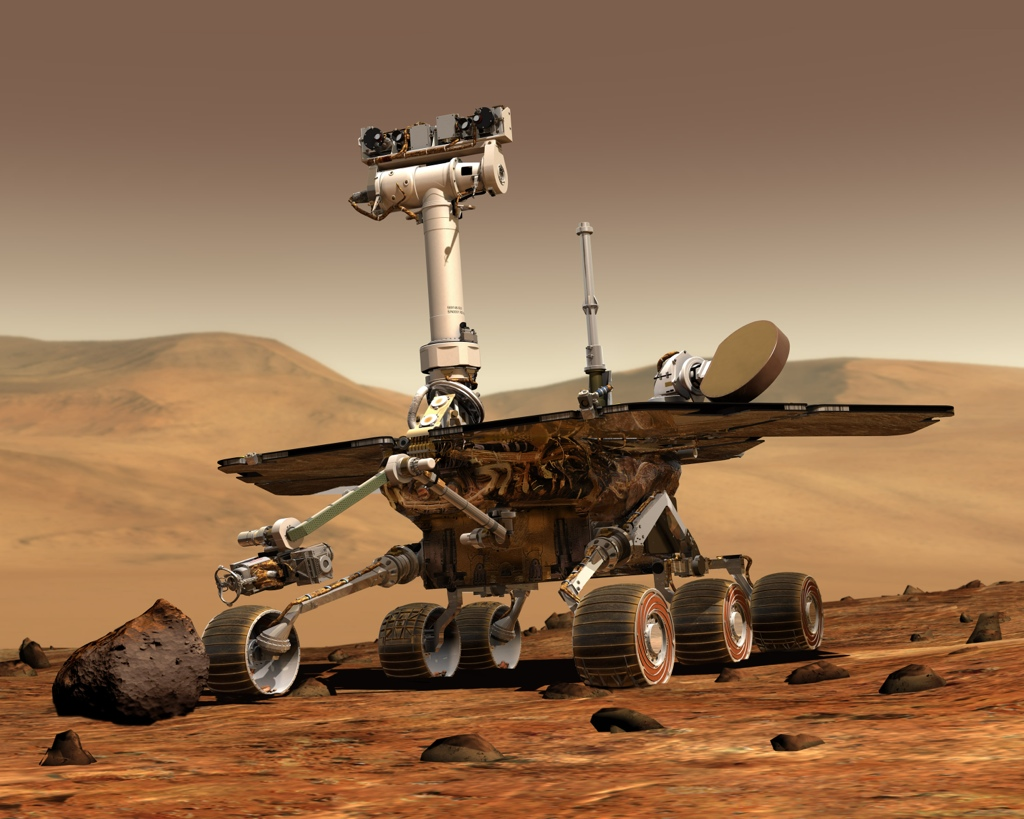
\includegraphics[width=6cm]{kapitel3/nasa_rover}
  \caption{Ein Nasa Rover}
  \label{Kap2:NasaRover}
\end{figure}

Man kann sich auch selbst ein Makro für das Einfügen von Bildern schreiben:

\bild{kapitel3/modell_point_to_point}{6cm}{Point to Point}

\begin{sidewaysfigure}
 \includegraphics[width=22cm]{kapitel3/ws-wsdl20-fehler}
  \caption{Sehr große Grafiken kann man drehen, damit sie auf die Seite passen}
  \label{Kap2:wsdl-fehler}
\end{sidewaysfigure}

Möchte man verhindern, dass Bilder in ein anderes Kapitel rutschen, steht der Befehl \verb+\clearpage+ zur Verfügung, der \LaTeX{} zwingt, alle bis dahin definierten \textit{floats} (Bilder, Tabellen, Formeln etc.) auszugeben.

\clearpage % Alle Bilder, die bisher kamen ausgeben


\section{Formelsatz}

Eine Formel gefällig? Mitten im Text $a_2 = \sqrt{x^3}$ oder als eigener Absatz (siehe \autoref{Formel}):

\begin{equation}
\begin{bmatrix}
   1 &  4 &  2 \\
   4 &  0 & -3
\end{bmatrix}
        \cdot
\begin{bmatrix}
   1 &  1 &  0 \\
  -2 &  3 &  5 \\
   0 &  1 &  4
\end{bmatrix}
       {=}
\begin{bmatrix}
  -7 &  15 &  28 \\
   4 &   1 & -12
\end{bmatrix}
\label{Formel}
\end{equation}

Wenn Ihre Formel zu breit für eine Zeile wird, können Sie sie mithilfe der \texttt{split}-Umgebung und einem doppelten Backslash (\verb+\\+) umbrechen.

\begin{equation}
\label{eq:4}
\begin{split}
\mathbf{F}_{{eigen}}=\sqrt[3]{\coprod_{i=1}^{3} \lambda_{i}},
\frac{\lambda_{1}-\lambda_{3}}{\lambda_{1}},
\frac{\lambda_{2}-\lambda_{3}}{\lambda_{1}},
\frac{\lambda_{3}}{\lambda_{1}} \\-
\sum_{i=1}^{3} \lambda_{i} \log \left(\lambda_{i}\right),
\frac{\lambda_{1}-\lambda_{2}}{\lambda_{1}}
\end{split}
\end{equation}

Sie können Formelelemente auch am Gleichheitszeichen ausrichten, hierzu dient die \texttt{align}-Umgebung:

\begin{align}
2x - 5y &=  8 \\
3x + 92y &=  -12
\end{align}

Wollen Sie keine Nummerierung der Formeln, ergänzen Sie einfach einen \texttt{*} bei den Namen der Umgebungen, d.h. Sie verwenden \texttt{equation*} oder \texttt{align*}.

\begin{equation*}
\begin{bmatrix}
   1 &  4 &  2 \\
   4 &  0 & -3
\end{bmatrix}
        \cdot
\begin{bmatrix}
   1 &  1 &  0 \\
  -2 &  3 &  5 \\
   0 &  1 &  4
\end{bmatrix}
       {=}
\begin{bmatrix}
  -7 &  15 &  28 \\
   4 &   1 & -12
\end{bmatrix}
\end{equation*}

\section{Zahlendarstellung und Angabe von Einheiten}
Zahlen und Einheiten können wie folgt angegeben werden: 

\begin{tabular}{|l|l|}
	\hline
	\textbf{Befehl} & \textbf{Ausgabe}  \\\hline
	\verb*|\num{123}| & \num{123} \\
	\verb*|\num{1234}| &	\num{1234} \\
	\verb*|\num{12345}| &	\num{12345} \\
	\verb*|\num{0.123}| &	\num{0.123} \\
	\verb*|\num{0,12345}| &	\num{0,1234} \\
	\verb*|\num{.12345}| &	\num{.12345} \\
	\verb*|\num{3.45d-4}| &	\num{3.45d-4} \\
	\verb*|\num{-e10}| &	\num{-e10} \\
	\verb*|\qty[per-mode=symbol]{2.8}{\giga\byte\per\second}| & \qty[per-mode = symbol]{2.8}{\giga\byte\per\second}\\
	\verb*|\qty[per-mode=fraction]{2.8}{\giga\byte\per\second}| & \qty[per-mode = fraction]{2.8}{\giga\byte\per\second}\\
	\verb*|\qty[mode=text]{2.8}{\giga\byte\per\second}| & \qty[mode = text]{2.8}{\giga\byte\per\second}\\\hline
\end{tabular}

\vspace*{0.75cm}

Listen können ebenfalls mit Einheiten versehen werden:\\ \verb*|\qtylist{10;30;45}{\giga\byte\per\second}| liefert die Ausgabe: \qtylist{10;30;45}{\giga\byte\per\second}. 

Bereiche können mit dem Befehl \verb*|\qtyrange{10}{30}{\giga\byte\per\second}| ausgegeben werden. \qtyrange{10}{30}{\giga\byte\per\second}


\section{Sourcecode}

Man kann mit Latex auch ganz toll Sourcecode in den Text aufnehmen.

\subsection{Aus einer Datei}

\lstinputlisting[firstline=2,                 % Erste anzuzeigende Zeile aus der Datei
                 language=Java,               % Programmmiersprache (für Highlighting)
                 caption={Crypter-Interface}, % Beschriftung
                 label=lst:CrypterInterface]  % Label (für Referenzen)
                 {\srcloc/Crypter.java}       % Pfad zur Datei, die angezeigt wird

Mit Zeilennummern

\lstinputlisting[numbers=left,                % Mit Zeilennummern auf der linken Seite
                 firstline=10,                % Erste anzuzeigende Zeile aus der Datei
                 lastline=15,                 % Letzte anzuzeigende Zeile aus der Datei
                 language=Java,               % Programmmiersprache (für Highlighting)
                 caption={Crypter},           % Beschriftung
                 label=lst:CrypterInterface2] % Label (für Referenzen)
                 {\srcloc/Crypter.java}       % Pfad zur Datei, die angezeigt wird


\subsection{Inline}

\begin{lstlisting}[language=Java,caption=Methode checkKey()]
    /**
     * Testet den Schlüssel auf Korrektheit: Er muss mindestens die Länge 1
     * haben und darf nur Zeichen von A-Z enthalten.
     *
     * @param key zu testender Schlüssel
     * @throws CrypterException wenn der Schlüssel nicht OK ist.
     */
    protected void checkKey(Key key) throws CrypterException {

        // Passt die Länge?
        if (key.getKey().length == 0) {
            throw new CrypterException("Der Schlüssel muss mindestens " +
                    "ein Zeichen lang sein");
        }

        checkCharacters(key.getKey(), ALPHABET);
    }
\end{lstlisting}


\section{Anforderungen}

Anforderungen im Format des Volere"=Templates (Snowcards) \autocite{Volere} können per Makro eingefügt werden. Das Label wird automatisch mit der Nummer erstellt, d.\,h. Sie können auf die Tabelle mit dieser referenzieren (siehe \autoref{F52}).

\snowcard % Snowcard einbinden (Anpassungen in titelblatt.tex)
   {F52} % Nummer des Requirements
   {F} % Art
   {Hoch} % Priorität
   {User Authentifizierung} % Titel
   {Interview mit Abteilungsleiter} % Herkunft (Optional)
   {F12} % Konflikte (Optional)
   {Der Benutzer ist in der Lage sich über seinen
    Benutzernamen und sein Passwort am System anzumelden} % Beschreibung
   {Ein Benutzer kann sich mit seinem firmenweiten Benutzernamen und
   Passwort über die Anmeldemaske anmelden und hat Zugriff auf die
   Funktionen des Systems} % Fit-Kriterium (Optional)
   {Benutzerhandbuch des Altsystems} % Material (Optional)

Ebenso können Sie nicht"=funktionale Anforderungen mit Hilfe von Quality Attribute Scenarios (vgl. \autoref{NF11}) darstellen. Zu Details siehe \autocite{Barbacci2003}.

\qas % Quality-Attribute Scenario einbinden (Anpassungen in titelblatt.tex)
   {NF11} % Nummer des Requirements
   {Hoch} % Priotität
   {Performance des Jahresabschlusses} % Titel
   {Endbenutzer} % Quelle
   {Startet einen Jahresabschluss} % Stimulus
   {Buchhaltungssystem} % Artefakt
   {Das System befindet sich im normalen Betriebszustand} % Umgebung
   {Jahresabschluss ist durchgeführt und kann als PDF abgerufen werden} % Antwort
   {10 Minuten} % Antwort-Maß

Die Abgrenzung von funktionalen und nicht-funktionalen Anforderungen ist nicht immer einfach und bereitet manchen Studierenden Probleme. Als Hilfestellung kann die von der ISO25010 \autocite{ISO25010} zur Verfügung gestellte Liste dienen, siehe \autoref{kapitel3/iso25010}.

\bild{kapitel3/iso25010}{14cm}{Qualitätsmodell für Software-Produkte nach ISO25010}

\citeauthor{Bass2003} listen in \autocite{Bass2003} eine ähnliche Liste von Kategorien für nicht-funktionalen Anforderungen auf, die ebenfalls als Richtschnur dienen kann. Diese sind:

\begin{itemize}
  \item \textit{Verfügbarkeit} \textit{(availability)} -- umfasst Zuverlässigkeit (reliability), Robustheit (robustness), Fehlertoleranz (fault tolerance) und Skalierbarkeit (scalability)
  \item \textit{Anpassbarkeit} \textit{(modifiability)}, umfasst Wartbarkeit (maintainability), Verständlichkeit (understandability) und Portabilität (portability).
  \item \textit{Performanz} \textit{(performance)}
  \item \textit{Sicherheit} \textit{(security)}
  \item \textit{Testbarkeit} \textit{(testability)}
  \item \textit{Bedienbarkeit} \textit{(usability)}
\end{itemize}
 % Externe Datei einbinden
% \chapter{Checkliste}
\label{Kap4}

Die folgende Checkliste kann dazu dienen, die Arbeit auf die wichtigsten Bewertungskriterien zu prüfen. Jeder Dozent hat andere Kriterien, die unten aufgeführten dürften aber für die meisten Dozenten gültig sein.

\section{Form und Sprache}

\begin{checklist}
  \footnotesize
  \item \textbf{Aufbau}: Die Arbeit ist nach wissenschaftlichen Prinzipien aufgebaut (wesentliche Teile vorhanden, Nummerierung/Verweise korrekt, Verzeichnisse vorhanden).
    \begin{checklist}
        \item \textit{Wesentliche Teile}: Die folgenden Elemente der Arbeit sind vorhanden: Titelblatt, Abstract/Zusammenfassung, Einleitung, Hauptteil, Fazit/Ausblick.
        \item \textit{Nummerierung/Verweise}: Das Nummerierungsschema wird konsistent über die gesamte Arbeit durchgehalten, die Verweise auf die verschiedenen Elemente (Abbildungen, Tabellen etc.) sind korrekt.
        \item \textit{Verzeichnisse}: Die Arbeit enthält alle relevanten Verzeichnisse: Inhaltsverzeichnis, Literaturverzeichnis, Abbildungsverzeichnis, Tabellenverzeichnis, eventuell Glossar.
    \end{checklist}
  \item \textbf{Sprache}: Die verwendete Sprache entspricht wissenschaftlichen Ansprüchen.
    \begin{checklist}
        \item \textit{Begriffe und Definitionen}: Begriffe werden einheitlich und konsistent verwendet. Neue Begriffe werden definiert und mit Literatur hinterlegt.
        \item \textit{Abkürzungen}: Alle Abkürzungen werden eingeführt und erläutert. Abkürzungen werden bei der ersten Verwendung ausgeschrieben und in einem Abkürzungsverzeichnis geführt. Es werden keine unüblichen oder selbst erfunden Abkürzungen verwendet. Ein Glossar kann verwendet werden, um Begriffe noch einmal kompakt darzustellen.
        \item \textit{Rechtschreibung}: Die Arbeit ist frei von Rechtschreibungs-, Zeichensetzungs- und Grammatikfehlern.
    \end{checklist}
  \item \textbf{Formatierung, Typografie}: Die Formatierung der Arbeit ist korrekt und aus typographischer Sicht einwandfrei. \textit{Wenn Sie dieses Template korrekt verwenden, sollte dieser Punkt automatisch durch die Verwendung von \LaTeX \ erledigt sein.}
    \begin{checklist}
        \item \textit{Korrekte Typografie}: Schriftarten werden korrekt verwendet (nicht mehr als 2 Fonts), der Zeilenabstand ist passend, die Ränder sind ausreichend, der Satz ist korrekt.
        \item \textit{Satz von Abbildungen, Tabellen etc.}: Abbildungen sind in der richtigen Auflösung dargestellt, die Tabellen sind korrekt gesetzt, mathematische Formeln und Symbole sind sauber dargestellt.
    \end{checklist}
  \item \textbf{Abbildungen}: Abbildungen werden in ausreichendem Umfang zur Förderung des Verständnisses eingesetzt. Sie werden korrekt im Text referenziert und sind, wo immer möglich, in einer Standardnotation erstellt.
    \begin{checklist}
        \item \textit{Ausreichende Verwendung}: Komplizierte Sachverhalte werden durch Abbildungen verdeutlicht. Es werden genug Abbildungen eingesetzt, um die wichtigsten Sachverhalte zu erklären.
        \item \textit{Verständnisförderung}: Abbildungen dienen nicht als Schmuck, sondern um komplizierte Sachverhalte zu verdeutlichen.
        \item \textit{Einbindung in den Text}: Der Text muss auch ohne Abbildungen verständlich sein, die Abbildungen helfen Sachverhalte aus dem Text besser darzustellen. Der Text referenziert die Abbildung korrekt.
        \item \textit{Standardnotation, Legende}: Die Abbildungen verwenden Standard"=Notationen wie UML, FMC etc. Wo keine Standardnotation eingesetzt wird, ist eine Legende vorhanden, um die Bildelemente zu erläutern.
    \end{checklist}
  \item \textbf{Zitate}: Quellen werden konsistent nach einer gängigen Zitierweise zitiert und sind vollständig im Literaturverzeichnis angegeben.
    \begin{checklist}
        \item \textit{Zitierweise}: Die Zitierweise in der gesamten Arbeit folgt einem einheitlichen Schema, z.B. IEEE, DIN, Chicago.
        \item \textit{Vollständigkeit}: Alle Zitate sind als solche kenntlich gemacht und die Quelle wird vollständig angegeben, und Plagiate werden vermieden.
    \end{checklist}
  \item \textbf{Schreibstil}: Lebendiger, wissenschaftlicher und verständlicher Schreibstil.
    \begin{checklist}
        \item \textit{Wissenschaftlichkeit}: Der Text ist im Präsenz geschrieben, es wird die dritte Person verwendet, Fachausdrücke werden korrekt verwendet, Fremdwörter und Amerikanismen werden richtig eingesetzt.
        \item \textit{Verständlichkeit}: Abschweifungen und Wiederholungen werden vermieden, statt dessen werden präzise und übersichtliche Sätze verwendet.
        \item \textit{Lebendigkeit}: Der Text der Arbeit zeichnet sich durch eine gute Wortwahl, Sprachbilder, einen angemessenen Satzbau und eine hohe Variabilität aus.
    \end{checklist}
\end{checklist}

\section{Inhalt}

\begin{checklist}
  \footnotesize
  \item \textbf{Gliederung}: Die Gliederung ist vollständig, konsistent und sachlogisch mit angemessener Struktur und Tiefe.
    \begin{checklist}
        \item \textit{Konsistenz und Vollständigkeit}: Auf einer Ebene stehen keine Punkte alleine, die Gliederungspunkte orientieren sich an der Argumentationskette.
        \item \textit{Angemessene Tiefe}: Die Größe der einzelnen Unterpunkte ist vom Umfang her ähnlich. Es gibt keine Gliederungspunkte, die nur aus ein bis zwei Sätzen bestehen.
    \end{checklist}
  \item \textbf{Grundlagen}: Es werden alle relevanten Grundlagen gelegt. Der State"=of"=the"=art und der State"=of"=practice werden dargelegt.
    \begin{checklist}
        \item \textit{Umfang}: 1/3 des Hauptteils ist ein gutes Maß für eine ausreichende Darstellung der Grundlagen.
        \item \textit{Begriffe und Methoden}: Begriffe und Methoden sind definiert, und Literatur zu den Definitionen ist angegeben.
        \item \textit{State-of-the-art}: Der Stand des verfügbaren Wissens wird dargestellt, analysiert und kritisch beurteilt (state-of-the-art). Bei theoretischen Arbeiten kann ein eigenes Kapitel \enquote{verwandte Arbeiten} nötig sein, um den state"=of"=the"=art darzustellen.
        \item \textit{State-of-practice}: Bei praktischen Arbeiten, die in der Industrie geschrieben werden, kann es nötig sein, auch das Vorgehen im Unternehmen zu erläutern.
    \end{checklist}
  \item \textbf{Methodik/Lösung}: Die gewählte Methodik bzw. Lösung ist für das Problem adäquat.
    \begin{checklist}
        \item \textit{Anforderungen an die Lösung}: Die von der Lösung zu erfüllenden Anforderungen werden dargestellt. Wo nötig wird dies auf Grundlage eines sauberen Requirements"=Engineerings durchgeführt.
        \item \textit{Erläuterung des Lösungsansatzes}: Der gewählte Lösungsansatz wird ausführlich erläutert und verständlich dargestellt.
        \item \textit{Eignung zur Lösung der Aufgabe}: Die gewählte Lösung ist geeignet, um das beschriebene Problem zu lösen.
        \item \textit{Hypothesen}: Es sind ggf. Hypothesen gebildet worden; diese sind erläutert, und es sind Kriterien identifiziert worden, mit deren Hilfe man die Hypothesen falsifizieren kann.
        \item \textit{Alternativen}: Es werden Alternativen zur vorgeschlagenen Lösung diskutiert. Die eigene Lösung wird nicht als einzige mögliche dargestellt, sondern es werden auch andere mögliche Lösungen vorgestellt und bewertet.
        \item \textit{Begründung}: Alternativen und Kriterien für die Auswahl dieser Lösung werden dargestellt.
        \item \textit{Vorteile der Lösung}: Es wird dargestellt, wieso die entwickelte Lösung vorteilhafter ist als die bisherigen Ansätze. Diese Darstellung erfolgt auf Basis des Lösungsansatzes. Eine konkrete Validierung der Implementierung erfolgt ggf. in späteren Kapiteln.
    \end{checklist}
  \item \textbf{Logik der Argumentationskette}: Die Argumentation ist logisch und nachvollziehbar. Sie ist frei von logischen Fehlschlüssen.
  \item \textbf{Implementierung}: Wenn eine Implementierung der Lösung erfolgt, so wird die Implementierung beschrieben. Die Darstellung der Implementierung kann knapp ausfallen. Wichtig ist der Lösungsansatz, nicht die konkrete Umsetzung.
  \item \textbf{Validierung}: Die vorgeschlagene Lösung wird ggf. empirisch verprobt.
    \begin{checklist}
        \item \textit{Vorgehensweise}: Die Vorgehensweise zur Validierung der Lösung / Hypothesen ist beschrieben und geeignet, relevante Aspekte der Lösung zu überprüfen.
        \item \textit{Empirische Analyse}: Die Erfassungsmethode wird dargestellt und die Daten werden nach den Grundsätzen ordnungsgemäßer Laborpraxis gesammelt und statistisch korrekt ausgewertet.
        \item \textit{Verprobung}: Die Lösung wird an einem praktischen Beispiel verprobt, und es werden wissenschaftlich korrekte Schlüsse aus der Anwendung gezogen.
        \item \textit{Zielerreichung}: Funktioniert die gewählte Lösung nach der Implementierung? Wie weit wurde das Ziel erreicht? Falls nicht, gibt es nachvollziehbare Gründe dafür und wurden diese dargestellt?
    \end{checklist}
  \item \textbf{Diskussion}: Die Lösung und ihre Validierung wird kritisch und im Kontext möglicher Alternativen diskutiert und bewertet.
    \begin{checklist}
        \item \textit{Kritische Reflexion}: Grenzen und Schwächen der eigenen Ergebnisse werden beleuchtet.
        \item \textit{Ableitung von Konsequenzen}: Die Konsequenzen aus den Ergebnissen für die Wissenschaft und Praxis sind beschrieben.
    \end{checklist}
  \item \textbf{Quellenarbeit}: Es werden hochwertige Quellen in ausreichendem Umfang genutzt und kritisch hinterfragt. Eventuell vorhandene Quellen aus dem Unternehmen werden ebenfalls berücksichtigt.
    \begin{checklist}
        \item \textit{Umfang}: Der Umfang an Quellen richtet sich stark nach Thema und Art der Arbeit. Bei einer Bachelorarbeit sind mindestens 20--30 Quellen üblich, bei einer Masterarbeit deutlich mehr.
        \item \textit{Wissenschaftliche Qualität}: Nicht zitierfähig sind Internet"=Quellen, Wikipedia"=Einträge sowie andere Bachelor- oder Masterarbeiten (sofern nicht veröffentlicht). Das ausschließliche Zitieren von Lehrbüchern ist problematisch. Aktuelle wissenschaftliche Artikel und Werke sollten in den Quellen auftauchen.
        \item \textit{Quellen \enquote{aus der Praxis}}: Wenn es im Unternehmen spezielle Quellen und Informationen gibt, so werden diese berücksichtigt, z. B. firmen- oder branchenspezifischer Informationen.
        \item \textit{Kritische Würdigung}: Quellen und Zitate werden kritisch hinterfragt und nicht einfach unreflektiert übernommen. Es gibt eine kritische Distanz bei der Quellenauswahl und Quellenauswertung.
    \end{checklist}
  \item \textbf{Fazit}: Es wird eine Zusammenfassung der Arbeit sowie Ausblick auf weitere mögliche Arbeiten im Themenfeld gegeben, etwa die Lösung ausstehender Probleme oder die Erfüllung zusätzlicher Anforderungen.
  \item \textbf{Umfang der Arbeit}: Richtgrößen: Bachelorarbeiten: 50--80 Seiten, Masterarbeiten: 60--100 Seiten, jeweils ohne Verzeichnisse und Anhang.
\end{checklist}

\section{Vor der Abgabe}

\begin{checklist}
  \footnotesize
  \item \textit{Korrektur}: Haben Sie einen Dritten die Arbeit lesen lassen und alle gefundenen Rechtschreib- und Zeichensetzungsfehler behoben?
  \item \textit{Literaturverzeichnis}: Sind im Literaturverzeichnis irrelevante Informationen entfernt? Beispielsweise bei Büchern unnötige Informationen über die Herkunft bei Google-Books oder bei Papern doppelte Angaben der DOI?
  \item \textbf{Abgabe auf Papier}
  \begin{checklist}
    \item \textit{Template passend eingestellt}: Haben Sie in der Datei \texttt{thesis.tex} eingestellt, dass Sie auf Papier abgeben wollen?
    \item \textit{Doppel- oder einseitiger Druck}: Entspricht die Einstellung des Templates dem Druck, d.\,h. ist das Template für doppelseitigen Druck eingestellt, wenn doppelseitig gedruckt werden soll und umgekehrt?
    \item \textit{Umschläge}: Sind die Umschläge vorhanden, um die Arbeit später zu binden? Die Umschläge können in der Hausdruckerei der Hochschule erworben werden.
    \item \textit{Copyshop}: Wissen Sie, wo Sie die Arbeit drucken werden? Die Hausdruckerei kann Ihre Arbeit nicht drucken.
    \item \textit{Exemplare}: Haben Sie geklärt, ob der Zweitkorrektor auch ein gedrucktes Exemplar möchte?
  \end{checklist}
  \item \textbf{Digitale Abgabe}
  \begin{checklist}
    \item \textit{Zustimmung des Betreuers/der Betreuerin}: Haben Sie mit Ihrer Betreuerin bzw. Ihrem Betreuer abgeklärt, dass Sie digital abgeben dürfen?
    \item \textit{Template passend eingestellt}: Haben Sie in der Datei \texttt{thesis.tex} eingestellt, dass Sie digital abgeben wollen?
    \item \textit{Unterschrift}: Haben Sie Ihre Unterschrift eingescannt und unter dem Namen \texttt{unterschrift.png} im Hauptverzeichnis abgelegt?
  \end{checklist}
\end{checklist}
 % Externe Datei einbinden


\chapter{The Purpose of the Project}
How might we help non-technical stakeholders to understand the value of telematics data with visualizations / dashboards?". Mit dieser Fragestellung beauftragte das Unternehmen Caruso GmbH zu Beginn des Wintersemesters 22/23 Gruppen von Studierenden der Hochschule Mannheim im Rahmen der Vorlesung "Projektsemester Software Enginnering" (PSE). Innerhalb von zwei Semestern wird eine Anwendung entwickelt, die den Entscheidungsprozess von Caruso's Kunden zum Kauf ihres Produktes anhand verständlicher Datenvisualisierung ermöglichen soll.

\section{The User Business or Background of the Project Effort}
Das Unternehmen Caruso stellt seit 2017 eine standartisierte Schnittstelle für Telemetriedaten für connected Cars verschiedener Hersteller bereit. Connected Cars sind Fahrzeuge die über Internetverbindung in der Lage sind, ihre phsyikalische gemessenen Daten (Telemetriedaten) wie Temperatur, oder Reifendruck zu versenden.

Caruso schließt Verträge mit Autoherstellern (OEMS) wie Mercedes oder BMW, Verträge zur Vernetzung von Autodaten über ihren Dienst ab. Die propertiären Fahrzeuginformationen werden erfasst und über eine einheitliche Schnittstelle, der Caruso API zur Verfügung gestellt. Diese Datenpunkte beinhalten informationen von der Position des Fahrzeugs oder dem nächsten Servicetermin. Die Datenpunkte werden in gebündelten Pakten, auch Datenpakten abonniert und abhängig von der Nutzung abgerechnet. Caruso verkauft die Datenpakte an Kunden wie Werkstätten, Versicherungen oder Pannendienste.

% Caruso Sales-Mitarbeiter Workflow??

Viele dieser Kunden sind mittelständische Unternehmen, welche den Mehrwert dieser Schnittstelle und der zur Verfügung gestellten Daten erkennen wollen, bevor sie in den Zugang zur Schnittstelle investieren. Caruso spricht in diesem Kontext von Entscheidungsträgern. Entscheidungstärger sind Personen in den Unternehmen, welche die Entscheidung zum Einkaufen des Produkts geben. In der Regel sind die Entscheidungsträger nicht technische Mitarbeiter ind Führugnspositionen, die mit den Rohdaten der Datenpunkte nichts anfangen können. Sie verlangen häufig Daten oder Versicherungen, welche über ihre Fahrzeuge gesammelt werden und leicht verständlich sind. Besonders Live-Inforamtionen über das Fahrzeug sind von Interesse.

Caruso stellt derzeit keine Anwendung bereit, die Live-Informationen verständlich für nicht technische Benutzer zur Verfügung stellt. Aktuell werden beispielsweise Skripte erstellt, welche die informationen der Fahrzeuge über die Schnittstelle sammeln und in einem Excel oder HTML-Bericht zur Verfügung stellen. Die Berichte werden in manuellen Prozessen durch mehrere Caruso-Mitarbeiter erstellt und müssen für jeden Kunden individuell erstellt werden.
\section{Goals of the Project}
Das übergeordnete Ziel für das gesamte Projekt lautet: "Durch einen verbesserten Workflow werden für den Entscheidungsträger relevante Daten schneller und verständlicher vom Sales-Mitarbeiter dargestellt". Damit ist gemeint, dass der Sales-Mitarbeiter einfacher und schneller Präsentationen für die Vorstellung beim Entscheidungsträger vorbereiten kann und diese von den Entscheidungsträgern besser verstanden werden. Konkrete lässt sich dieses Ziel in mehrere Subziele einteilen:
\begin{itemize}
  \item 1. Das Produkt visualisiert Live-Informationen der Fahrzeuge. Dies erhöht das Vertrauen der Entscheidungsträger in das Caruso-System.
  \item 2. Das Produkt zeigt die Datenpunkte für nicht-technische Entscheidungsträger verständlich an. Dies sorgt dafür, dass der Mehrwert der Daten sichtbarer wird.
  \item 3. Das Produkt ist wiederverwendbar für mehrere Entscheidungsträger. Dies sorgt dafür, dass der Zeitaufwand für eine manuelle Datensammlung seitens Caruso minimiert wird.
  \item 4. Das Produkt enthält eine leicht verständliche konfiguration. Dies sorgt dafür, dass die nicht-technischen Mitarbeiter von Caruso keine Hilfe von Entwicklern der Caruso GmbH benötigen.
\end{itemize}

\section{Overall Solution}
Die grobe Lösung für die Fragestellung von Caruso ist eine webbasierte Anwendung in Form mehrere Dashboards. Diese lassen sich für einzelne Entscheidungsträger konfigurieren. Sie beinhalten die Informationen der Kundenfahrzeuge in Form visualisierter Datenpunkte sowohl für einzelne Fahrzeuge als auch Gruppen von Fahrzeugen (Flotten).
\chapter{The \Glspl{stakeholder}}
In this chapter, we will identify the key \glspl{stakeholder} of the project and describe their needs, expectations, and concerns as they relate to the project. By understanding the needs and expectations of our \glspl{stakeholder}, we can ensure that the project meets their requirements and delivers the desired outcomes.
\begin{figure}[ht]
  \centering
  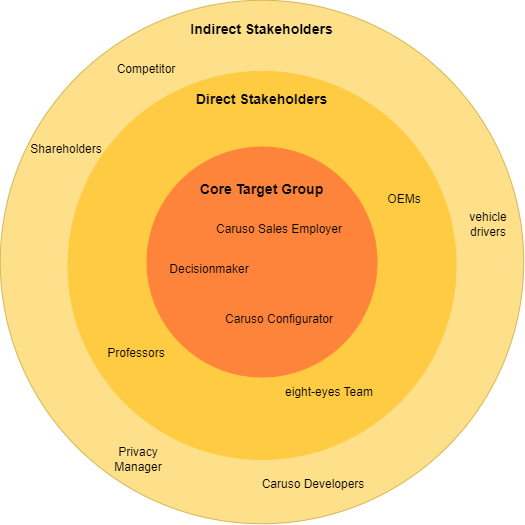
\includegraphics[width=\textwidth]{stakeholders/stakeholders.png}
  \caption{\Glspl{stakeholder} map containing the prioritised  \glspl{stakeholder} for the project}
  \label{Kap2:Stakeholders}
\end{figure}
Figure \ref{Kap2:Stakeholders} shows the \glspl{stakeholder} of the project. \Glspl{stakeholder} are separated into three categories: the core target group, direct \glspl{stakeholder} and indirect \glspl{stakeholder}. The core target group are the main beneficiaries of Carvis, the people who are intended to use the product. The direct \glspl{stakeholder} are people and organisations who are linked to the project. They either work on the project or provide critical information without which it could not succeed. The indirect \glspl{stakeholder} are people and organisations who also profit from the success of the project but have no direct impact on it.

\section{Core Target Group}
The core target group consists of three \glspl{stakeholder}: the Caruso sales employee, the Caruso configurator and the decision maker of a potential customer company. The following section will present the obligations of each \gls{stakeholder} and explain their relevance to the project.

\subsection{The Sales Employee}
The Caruso sales employee is a representative of Caruso who negotiates and closes contracts with decision makers of other companies and sells them Caruso services. Their obligations include:
\begin{itemize}
  \item the acquisition of customers,
  \item the preparation of sales pitches for decision makers,
  \item the presentation of the sales pitch to build the decision maker's trust in Caruso data,
  \item the answering of any remaining questions the decision maker may have,
  \item the preparation of customer-specific \glspl{data},
  \item and the closing of contracts with decision makers.
\end{itemize}
The Caruso sales employee is essential both in the current and the planned future process of acquiring new customers. They were the main point of contact for questions during the \glspl{sprint}.

\subsection{The Decision Maker}
Decision makers are potential customers of Caruso which are interested in the data provided. They are often the executives of medium-sized companies which hope to improve the workflow in their company or develop new applications using Caruso data. According to Caruso, the most profitable customers are insurances, roadside assistance companies and fleet management companies. During the \glspl{sprint}, contact to the decision makers wasn't established directly but their wishes were expressed by the sales employee. Still, their interests are a core driver in the design of the product as it is ultimately intended to convince them to invest in Caruso services. They:
\begin{itemize}
  \item decide whether or not to enter into contracts with Caruso on behalf of their companies,
  \item often have little technical know-how,
  \item and will only buy a product whose value they appreciate and which they trust.
\end{itemize}

\subsection{The Configurator}
The Caruso configurator is an employee which aggregates customer data into an Excel or HTML report. They have technological skill and will prepare the data for sales pitches at the request of the sales employee. Their obligations are:
\begin{itemize}
  \item the aggregation of vehicle data,
  \item the creation of Excel or HTML reports,
  \item and the manual configuration of reports to accommodate a decision maker's individual requests and wishes.
\end{itemize}
After the successful conclusion of this project, the configurator will have a much smaller role or will not be needed at all as Carvis will automatically aggregate the required data and will provide an interface for the sales employee to configure it without needing technical know-how. The configurator is part of the core target group because he is currently responsible for creating all forms of visualisation for the decision maker.

\section{Other \Glspl{stakeholder}}
The other \glspl{stakeholder} of the project are the direct and indirect \glspl{stakeholder}. As they are not directly responsible for any requirements of the project, they will not be mentioned in the following chapters and will only briefly be described here.

\subsection{Direct \Glspl{stakeholder}}
\begin{itemize}
  \item \textbf{The eight eyes Team}: The eight eyes team has identified Caruso's wishes and the requirements for an application to fulfil them. This resulting document will provide developers the basis for a successful project.
  \item \textbf{The Professors}: The professors established the first contact to Caruso and organised the central aspects of the project as part of the PSE course.
  \item \textbf{The \glspl{oem}}: The \glspl{oem} provide the raw vehicle data which Caruso buys and standardises. Without them, this project would not be possible.
\end{itemize}

\subsection{Indirect \Glspl{stakeholder}}
\begin{itemize}
  \item \textbf{The Shareholders}: The shareholders invest in Caruso and thus profit from any new contracts that may be closed as a result of the success of this project.
  \item \textbf{The Competition}: The competition are companies which offer similar services to Caruso. They will be negatively impacted by this projects success.
  \item \textbf{The Drivers}: The drivers are the customers of the decision makers. They will profit if the further use of Caruso data leads to better customer service or new applications they might use.
  \item \textbf{The Caruso Development Team} The development team will expand and maintain the Carvis system in the future.
  \item \textbf{The Data Security Officer}: Data security officers handle the security of Caruso data. Caruso cares about the security of their customer data, however according to Caruso it should not be a priority for the purposes of this project.
\end{itemize}

\section{\Glspl{persona}}
A representative \gls{persona} has been created for each \gls{stakeholder} of the core target group to better understand and gain deeper insight into their challenges. These \glspl{persona} include demographic information, a job description, goals, aspirations and challenges they face at work. It also describes how Carvis will support them to overcome their challenges and meet their goals.

\begin{figure}[ht]
  \centering
  \includegraphics*[width=\textwidth]{./Cornelius.pdf}
  \caption{\Gls{persona}: Sales Employee }
  \label{Persona:Cornelius}
\end{figure}
Figure \ref{Persona:Cornelius} shows "Cornelius von Grünwald" who is representative of the sales employee. As such it is his job to acquire new customers and hold presentations to showcase Caruso data. He has little technical know-how and relies on developers (configurators) to prepare data for him. He prioritises building trust between him and his customers and values their individual wishes.

\begin{figure}[ht]
  \centering
  \includegraphics*[width=\textwidth]{./Rube.pdf}
  \caption{\Gls{persona}: Decision Maker}
  \label{Persona:Rube}
\end{figure}
Figure \ref{Persona:Rube} shows "Rüdiger Rübe" who is representative of the decision maker of a fleet management company. He is the CEO of a medium-sized taxi company called EuroTaxi. He is interested in expanding his business with innovative technologies, however he needs to first be convinced of their use as every investment is a big risk in terms of time and resources spent. As he  has little technical knowledge and little time, \glspl{data} need to be presented in a simple and engaging way. 

\begin{figure}[ht]
  \centering
  \includegraphics*[width=\textwidth]{./annie.pdf}
  \caption{\Gls{persona}: Configurator}
  \label{Persona:Annie}
\end{figure}
Figure \ref{Persona:Annie} shows "Annie Ainsley" who is representative of the configurator. She is a senior Caruso developer who is intimately familiar with the \gls{api} and \glspl{data}. She is often asked by Cornelius to prepare data for him which takes time away for other tasks. She is also not familiar with Rüdiger or other decision makers and can't cater to their wishes well, so she has to be in close contact with Cornelius while she prepares the data for him.
\chapter{Constraints}

In this chapter, we will explore the constraints that must be considered in the design of our product. These constraints represent limitations that apply to the entire product, and must be taken into account no matter how we choose to solve the problem at hand. In this section, we will discuss the description, rationale, and fit criterion for each constraint, and how they are written in the same format as functional and non-functional requirements. Understanding and adhering to these constraints will be crucial to the success of this project.

\section{Partner or Collaborative Applications}

This chapter explores applications that the product will collaborate with, namely the \gls{dataplace}. By examining these partner applications, we can identify potential integration issues and design constraints. The dataplace can be found \href{https://www.caruso-dataplace.com/developer-zone/}{\emph{here}}\footnote{https://www.caruso-dataplace.com/developer-zone/}.

% Examples of these applications can be provided through descriptions, models, or references to specifications that include all interfaces impacting the product
As Carvis is a data appetiser for connected car data provided by Caruso, this constraint affects the data sources and the type of data that can be used. As the data provided by Caruso is ever evolving it is best to check the available \glspl{data} on the \gls{dataplace} platform. 

% \gls{dataplace}
% only use data for cars supported by caruso
The \gls{dataplace} provides a data catalogue and a \gls{api} documentation. The data catalogue provides a list of all available \glspl{data} and their description. The \gls{api} documentation provides a list of all available \gls{api} endpoints and their description and examples. The data catalogue and the \gls{api} documentation are available on the \gls{dataplace} developer zone. The data provided by Caruso is only available for cars that are supported by Caruso. The list of supported cars is available on the \gls{dataplace}.

\section{Schedule Constraints}

% wir haben uns auf einen usecase (flottenmanagement) konzentriert
Time is a constraint imposed by the nature of this project as a student project. This constraint largely affects the content of the application, as it limits the resources we have in terms of the \glspl{widget} we can include. In order to manage this constraint, we have focused on the fleet management \gls{usecase}, which includes \glspl{widget} that are relevant for all \glspl{usecase}.

By focusing on the fleet management \gls{usecase}, we have been able to maximize the resources we have within the given time frame and create a product that meets the needs of our \glspl{stakeholder} to the best of our ability. This enables to deliver a product that can be used in a production environment.

% TODO: maybe include the image of caruso showing the most important usecases to highlight why whe chose fleet management


\section{Budget Constraints}
% gibt keine Budget Constraints (Bezug auf 3b. nehmen)
% Description: The product shall not be subject to budget constraints.
% Rationale: This is a demo application that will only be used for a short time frame, and as such, budget constraints do not need to be considered.
% Fit criterion: The product shall not exceed the allocated budget for the demo application.

One constraint that we will not need to consider in the design of our product is budget constraints. Because this is a demo application that will only be used for a short time frame per user. As such, we do not need to worry about staying within a specific budget. By not having to worry about budget constraints, we will have more flexibility in our design choices and can focus on creating a product that meets the needs and expectations of the \glspl{stakeholder}.
\chapter{Relevant Facts and Assumptions}

% facts and assumptions that are not constraints or requirements. E. g. intresting information, delining the context.
There are a wide variety of customers that Caruso is looking to acquire. \autoref{caruso-customers} shows which of them are the most valuable customers. Carvis should mainly focus on those in the top right corner, as they are the best prepared and represent the highest yield opportunity.

\begin{figure}[ht]
  \centering
  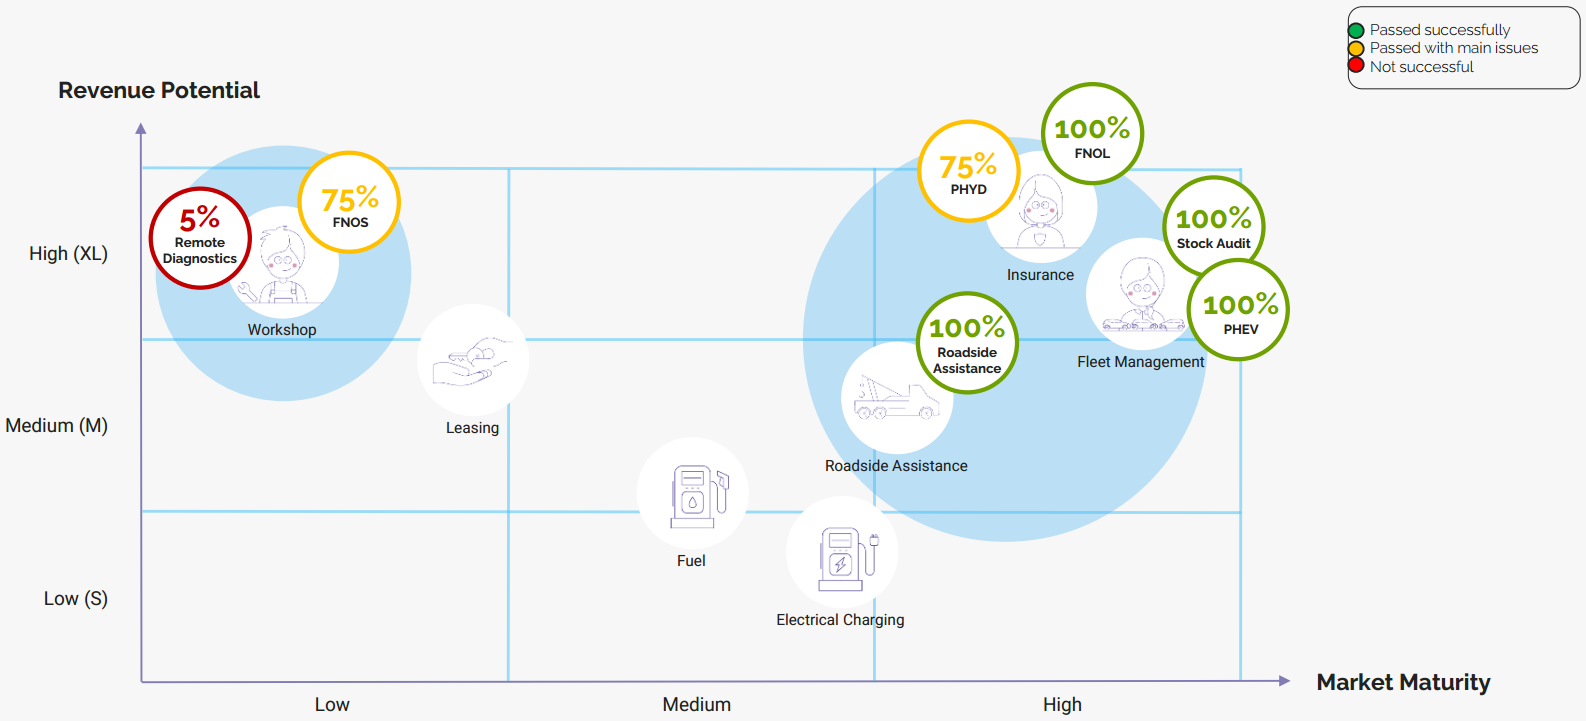
\includegraphics[width=\textwidth]{relevant_facts_and_assumptions/caruso-use-cases.png}
  \caption{Graph of different Caruso customers, they are ordered by revenue potential and market maturity.}
  \label{caruso-customers}
\end{figure}

A possible conclusion to the aforementioned statement could be that only large companies are compelling customers, which is not the case. Large companies have a lot of resources to invest in innovative technologies, so the demand for a data appetizer is lower. On the other hand mid-sized companies typically want to know what they are investing their money and time before allocating resources. This is where Carvis helps to highlight areas where Caruso data can be used.

Widgets designed as part of this project where not designed in cooperation with decision makers, instead the input of the Caruso sales employee was used. As a result of this, it is not certain that the widgets fit the needs of the specific use cases. The process of adjusting the widgets is the responsibility of the configurator. Talking to the decision makers is not part of the scope of this project.

The goal of this project is to deliver a finished product that meets the needs of our stakeholders, including Caruso. We understand that Caruso may not want to invest additional development time on their team to make adjustments to the application. As such, a modular system using widgets is the best solution for this project.
\chapter{The Scope of the Work}

This chapter describes important aspect to consider when building a new product. It determines the boundaries of the business area to be studied and outlines how it fits into its environment. Understanding the scope of the work and its constraints allows to establish the scope of the product and ensure that it will fit seamlessly into its intended environment.

In this document, we will delve into the current situation and the context of the work in order to fully understand the scope of the project. The current situation includes an analysis of the existing business processes, that will be changed by the Carvis. The context of the work, on the other hand, identifies the boundaries of the work that need to be investigated in order to build the product. This includes understanding the adjacent systems and their interfaces with the work context, as well as the details of when, how, where, who, what, and why they produce the necessary information. By understanding both the current situation and the context of the work a clear and comprehensive scope for the project can be established.

\section{The Current Situation}
The current way of acquiring new customers is shown in figure \ref{ScopeOfWork:Situation}.
\begin{figure}[ht]
  \centering
  % TODO neu in TikZ erstellen
  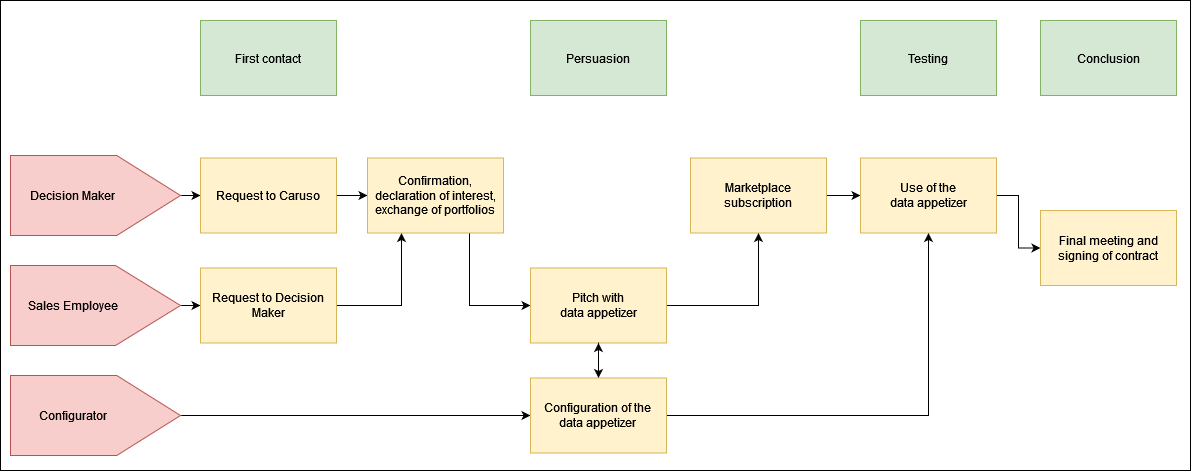
\includegraphics[width=\textwidth]{scope_of_the_work/current_situation.PNG}
  \caption{\Glspl{stakeholder}}
  \label{ScopeOfWork:Situation}
\end{figure}

Entry into a new contract currently requires three \glspl{stakeholder}: a decision maker, a Caruso sales employee and a Caruso configurator. The process can be split into four steps: first contact, persuasion, testing and conclusion. During first contact, the decision maker and sales employee enter into contact with each other. The sales employee gauges a decision makers interest in Caruso services or a decision maker becomes aware of Caruso through advertising, word of mouth or some other means.

After contact is established, the sales employee of Caruso holds a meeting with one or multiple decision makers. Here \glspl{data} of publicly accessible cars, Caruso vehicles or dummy cars are presented. For this purpose, a manually created HTML or Excel report of aggregated vehicle data of past rides is used. These include data such as distance driven per day of the week for an entire fleet of cars.

After the sales pitch, the decision makers trusts and wants to use Caruso's services. They can then create an account in the \gls{dataplace} and receive the aggregated data shown during the presentation to look at for themselves. This data usually isn't live.

After the decision makers are convinced of the value of the data, a final meeting is held where any open questions can be discussed with the sales employee. Finally, a contract is entered by the two parties.

\section{The Context of the Work}
Figure \ref*{ScopeOfWork:ContextDiagram} shows the communication between the core target group, the Carvis and the neighbouring systems in the form of a context diagram.

% TODO in TikZ neu erstellen
% TODO Konfigurator unter Sales Employee
\begin{figure}[ht]
  \centering
  \includegraphics*[width=\textwidth]{./context_diagram.png}
  \caption{Context Diagram}
  \label{ScopeOfWork:ContextDiagram}
\end{figure}

The decision maker has access to both the \gls{dataplace} and Carvis. The access to the \gls{dataplace} is required as the decision maker needs to create an account and register vehicles before they can access Carvis.

The sales employee uses Carvis to present Caruso data to the decision maker. They are not allowed to access the decision makers data but can use placeholder cars publicly accessible in the \gls{dataplace}. He also uses Carvis to configure projects for different decision makers. The configurator has no part in this proposed system because the sales employee will handle all forms of configuration without requiring much technical knowledge.
% TODO ausformulieren?
\chapter{The Scope of the Product}
In diesem Kapitel werden die einzelnen Anwendungsfälle des Produkts vorgestellt. Dabei werden die Rollen des Entscheidungsträgers, Sales Mitarbeiters und Konfigurators betrachtet. Anschließend werden Beschreibungen für die einzelnen Uses Case aufgeführt und für jeden der Anwendungsfälle ein Walkthrough in Form eines High fidelity Prototypen dargestellt.
\section{Product Boundary}
Die folgende Abbildung \ref{SopeOfProduct:ContextDiagram} zeigt ein Anwendungsfalldiagramm für die Stakeholder der Core Target Group und ihren individuellen Anwendungsfällen mit dem Produkt Carvis. Alle Use Cases sind mit einer Id versehen, welche über die weiteren Kapitel referenziert werden.
\begin{figure}[H]
  \centering
  \includegraphics*[width=\textwidth]{./use_case_diagram.png}
  \caption{Use Case Diagram}
  \label{SopeOfProduct:ContextDiagram}
\end{figure}
\section{Use Case Table}
\sffamily
\begin{footnotesize}
  \renewcommand{\arraystretch}{1.4}
  \begin{longtable}[i i i L]{ p{.1\textwidth} p{.2\textwidth} p{.16\textwidth} p{.44\textwidth} }
    \caption                       % Caption für das Tabellenverzeichnis
        {Use Case Table} % Caption für die Tabelle selbs
        \\
    \toprule
    \textbf{UC ID} & \textbf{UC Name} & \textbf{Actors}  & \textbf{Description}\\
    \midrule
    \hypertarget{Ref:UC1}{UC\_1} & View vehicle information & Decision Maker, Sales Employee & Der Decision Maker/Sales Employee wählt ein Fahrzeug aus und sieht sich die vorhandenen Information an. \\
    \hypertarget{Ref:UC2}{UC\_2} & View all vehicles & Decision Maker, Sales Employee & Der Decision Maker/Sales Employee sieht in einer Liste alle Fahrzeuge für sein Projekt. \\
    \hypertarget{Ref:UC3}{UC\_3}  & View fleet information & Decision Maker, Sales Employee & Der Decision Maker/Sales Employee sieht Statistiken über alle Fahrzeuge in seiner Flotte. \\
    \hypertarget{Ref:UC4}{UC\_4}  & Choose project & Sales Employee & Der Sales Employee wählt das Projekt aus, für das er seine Präsentation halten will. \\
    \hypertarget{Ref:UC5}{UC\_5}  & Create template & Configurator & Der Configurator erstellt ein Template seines Projekts, um dieses für zukünftige Projekte wiederverwenden zu können. \\
    \hypertarget{Ref:UC6}{UC\_6} & Choose template & Configurator & Der Configurator wählt ein Template für ein Projekt aus, um diesem eine Vorkonfiguration zuzuweisen. \\
    \hypertarget{Ref:UC7}{UC\_7} & Delete template & Configurator & Der Configurator löscht ein Template. \\
    \hypertarget{Ref:UC8}{UC\_8} & Delete project & Configurator & Der Configurator löscht ein Projekt, um seine aktiven Projekte aktuell zu halten. \\
    \hypertarget{Ref:UC9}{UC\_9} & Create project & Configurator & Der Configurator erstellt ein Projekt für einen neuen Entscheidungsträger. \\
    \hypertarget{Ref:U10}{UC\_10} & Reset project & Configurator & Der Configurator setzt ein Projekt zurück, um die Konfiguration neu zu beginnen. \\
    \hypertarget{Ref:UC11}{UC\_11} & Edit project & Configurator & Der Configurator bearbeitet den Projektnamen sowie die anzuzeigenden fahrzeugspezifischen Datenpunkte. \\
    \bottomrule
  \end{longtable}
\end{footnotesize}
\rmfamily

\section{Individual Product Use Cases}
Um den Ablauf der Use Cases besser zu verstehen, werden für alle Use Cases Abbildungen des Prototypen gezeigt, der im Laufe des Design Sprints erstellt wurde, um die Anforderungen zu erheben. Der Prototyp besteht aus zwei Perspektiven. Die erste Perspektive ist die Ansicht des Entscheidungsträgers, wenn er mit der Anwendung inteagiert. Die zweite Ansicht ist die es Sales Mitarbeiter und Konfigurators des Systems. Im Folgenden werden die einzelnen Ansichten des Prototypen aus der Perspektive des Entscheidungsträgers gezeigt.


\subsection{Perspektive des Entscheidungsträgers}
\begin{figure}[H]
  \centering
  \includegraphics*[width=\textwidth]{./prototyp/Default-View.png}
  \caption{Perspektive Entscheidungsträger: Startseite}
  \label{DecisionMaker:Homepage}
\end{figure}

Die Abbildung \ref{DecisionMaker:Homepage} zeigt die initiale Situation, aus welcher der Entscheidungsträger immer startet, nachdem er sich mit seinen Accountinformationen an der Applikation anmeldet. Auf dieser Seite wird der Use Case \hyperlink{Ref:UC2}{UC\_2} durchgeführt und die Möglichkeit der Ablauf für die Use Cases \hyperlink{Ref:UC1}{UC\_1} und \hyperlink{Ref:UC3}{UC\_3} ermöglicht. 


\subsubsection{Use Case 2: View all vehicles}
Das Szenario beginnt auf der initialen Ansicht in Abbildung \ref{DecisionMaker:Homepage}. Der Entscheidungsträger oder Sales Mitarbeiter sieht auf dieser Seite eine Tabelle mit mehreren Spalten, die alle Fahrzeuge beinhaltet, welche mit seinem Caruso-Marketplace-Konto verbunden sind. Die Tabelle beinhaltet mehrere Spalten zur genaueren Identifaktion der Fahrzeugs, beispielsweise den Hersteller oder den Status. Die Fahrzeuge lassen sich mit einem Klick auf den Spalten in aufsteigender oder absteigender Reihenfolge sortieren, damit die Fahrzeuge schnell gruppiert werden können. Außerdem ist es möglich spezifische Fahrzeuge zu suchen oder anhand der Filteroptionen Fahrzeuge auszublenden, die nicht betrachtet werden sollen.

\subsubsection{Use Case 1: View vehicle information}
Das Szenario beginnt auf der initialen Ansicht in Abbildung \ref{DecisionMaker:Homepage}. Der Entscheidungsträger oder der Sales Mitarbeiter wählt ein Fahrzeug über die Tabelle der Fahrezeuge aus. Wahlweise geschieht dies, nachdem ein Fahrzeug gesucht oder gefiltert wurde. Daraufhin befindet er sich auf der Fahrezugansicht in Abbildung \ref{DecisionMaker:DetailsRube}.

\begin{figure}[ht]
  \centering
  \includegraphics*[width=\textwidth]{./prototyp/Details-Rübe.png}
  \caption{Perspektive Entscheidungsträger: Fahrzeugansicht}
  \label{DecisionMaker:DetailsRube}
\end{figure}

Auf dieser Seite befinden sich alle Fahrzeuginformationen, zu dem vorher ausgewählten Fahrzeug. Die Datenpunkte, die von Caruso für das Fahrezeug zur Verfügung gestellt werden, sind in Weißen Kästchen, sogenannten Widgets zusammengefasst und logisch gruppiert. Ein Beispiel für solch ein Widget ist die allgemeine Fahrzeuginformation mit der VIN und dem Hersteller des Fahrzeugs. Jedes Widget beinhaltet eine Information darüber, wann das letzte Mal eine Aktualisierung durchgeführt wurde, damit der Entscheidungsträger weiß, wie aktuell die Daten sind. Für den Fall, dass manche Datenpunkte vom Hersteller nicht an Caruso geliefert werden und somit das Widget keine Informationen anzeigen kann, wird eine entsprechende Information erscheinen, wie in Abbildung \ref{DecisionMaker:NotSupported}.


\begin{figure}[ht]
  \centering
  \includegraphics*[width=5cm]{./prototyp/Not-Supported.png}
  \caption{Perspektive Entscheidungsträger: Nicht unterstützter Datenpunkt}
  \label{DecisionMaker:NotSupported}
\end{figure}

\subsubsection{Use Case 3: View fleet information}
Das Szenario beginnt auf der initialen Ansicht in Abbildung \ref{DecisionMaker:Homepage}. Von dieser Seite klickt der Entscheidungsträger oder der Sales Mitarbeiter auf den Reiter Flottenstatistik. Daraufhin öffnet sich die Ansicht auf Abbildung \ref{DecisionMaker:Fahrzeugstatistik}.
\begin{figure}[H]
  \centering
  \includegraphics*[width=\textwidth]{./prototyp/Fahrzeugstatistik.png}
  \caption{Perspektive Entscheidungsträger: Fahrzeugstatistik}
  \label{DecisionMaker:Fahrzeugstatistik}
\end{figure}
Auf dieser Seite befinden sich die flottenspezifischen Informationen aller registrieten Fahrzeuge in Form von Widgets. Wie auch in der Listenansicht ist hier das Filtern und Suchen möglich.

Die Widgets beinhalten beispielsweise eine Karte mit der Position aller Fahrzeuge, eine Statistik über die Hersteller der Fahrzeuge oder eine Liste mit vergangenen Ereignissen der Fahrzeuge. 

Zusätzlich zum Aktualisierungszeitpunkt geben diese Widgets ebenfalls an, wie viele Fahrzeuge die notwendigen Datenpunkte für das Widget liefern. Dies erhöht das Verständnis bei der Interpretation der Daten, da die genaue Menge an verwendeten Fahrzeugen bekannt ist.

\newpage
\subsection{Perspektive Sales Mitarbeiter und Konfigurator}

\begin{figure}[ht]
  \centering
  \includegraphics*[width=\textwidth]{./prototyp/Project-Selection.png}
  \caption{Perspektive Entscheidungsträger: Fahrzeugansicht}
  \label{Configurator:ProjectSelection}
\end{figure}
Die Abbildung \ref{Configurator:ProjectSelection} zeigt die initiale Situation, aus welcher der Sales Mitarbeiter oder der Konfigurator starten, wenn sie sich erfolgreich am System angemeldet haben. Auf dieser Seite werden die Use Cases \hyperlink{Ref:UC4}{UC\_4},  \hyperlink{Ref:UC5}{UC\_5},  \hyperlink{Ref:UC6}{UC\_6},  \hyperlink{Ref:UC7}{UC\_7}, \hyperlink{Ref:UC8}{UC\_8},  \hyperlink{Ref:UC9}{UC\_9},  \hyperlink{Ref:UC10}{UC\_10} und  \hyperlink{Ref:UC11}{UC\_11} begonnen.

\subsubsection{Use Case 4: Choose project}
Das Szenario beginnt auf Abbildung \ref{Configurator:ProjectSelection}. Der Sales Mitarbeiter sieht die vorhandenen Projekte in Form von weißen Kacheln. Diese beinhalten Informationen über den Namen der Firma, sowie Informationen über die letzte Einsicht oder die letzte Änderung. Anhand des Namens oder Alternativ der Suchfunktion findet der Sales Mitarbeiter Das Projekt, für das er eine Präsentation durchführen will. Dafür klickt er auf die enstprechende Projektkachel. Im Anschluss öffnet sich die Ansicht ähnlich wie in Abbildung \ref{DecisionMaker:Homepage}. Damit ist das Projekt ausgewählt.

\subsubsection{Use Case 5: Create template}
Das Szenario beginnt auf Abbildung \ref{Configurator:ProjectSelection}. Der Konfigurator wählt ein Projekt aus, welches er als Vorlage speichern will. Dafür klickt er auf die drei vertikalen Punkten in der rechten oberen Ecke der Projektkachel. Daraufhin verändert sich die Projektkachel zu der Abbildung \ref{Configurator:ProjectTileEdit}.

\begin{figure}[ht]
  \centering
  \includegraphics*[width=5cm]{./prototyp/ProjectTileEdit.png}
  \caption{Perspektive Configurator: Projektkachel editieren}
  \label{Configurator:ProjectTileEdit}
\end{figure}
Der Konfigurator klickt als Vorlage speichern. Daraufhin erscheint eine Möglichkeit einen Namen für die Vorlage zu vergeben und die Vorlage wird erstellt.

\subsection{Use Case 9: Create project}
Das Szenario beginnt auf Abbildung \ref{Configurator:ProjectSelection}. Der Konfigurator klickt auf die Projektkachel mit der Aufschrift Projekt erstellen.Daraufhin öffnet sich ein Popup wie in Abbildung \ref{Configurator:CreateProjectPopup}. 
\begin{figure}[ht]
  \centering
  \includegraphics*[width=7cm]{./prototyp/Projekt-Erstellen-Popup.png}
  \caption{Perspektive Entscheidungsträger: Fahrzeugansicht}
  \label{Configurator:CreateProjectPopup}
\end{figure}
Hier trägt der Konfigurator ein Dataplace-Konto ein, welches er mit dem Projekt verknüpfen will, sowie weitere Dataplace-Konten die in der Lage sein sollen, dieses Projekt einsehen zu können. Außerdem fügt er das Logo für des Unternehmens sowie deren beiden Hauptfarben zur Personalisierung hinzu. Anschließend klickt der Konfigurator auf Speichern, worauf sich eine Liste mit Vorlagen wie in Abbildung \ref{Configurator:Template} öffnet, aus denen das Projekt intial erstellt wird.

\begin{figure}[ht]
  \centering
  \includegraphics*[width=\textwidth]{./prototyp/Project-Selection-1.png}
  \caption{Perspektive Entscheidungsträger: Fahrzeugansicht}
  \label{Configurator:Template}
\end{figure}
In der Liste kann zusätzlich ein Vorlage über die Suche gefunden werden. Die Vorlagen besitzen eine Vorschau, damit der Konfigurator vor der Auswahl sieht, ob er sich für diese Vorlage entscheiden will. Der Konfigurator klickt eine Vorlage an. Daraufhin ist das Projekt erstellt.

\subsection{Use Case 8: Delete project}
Das Szenario beginnt in der Abbildung \ref{Configurator:ProjectSelection}. Der Konfigurator klickt auf die drei vertikalen Punkte in der rechten oberen Ecke des Projekts, dass er löschen will. Daraufhin verändert sich die Projektkachel wie in Abbildung \ref{Configurator:ProjectTileEdit}. Der Konfigurator klickt auf Löschen. Daraufhin ist das Projekt gelöscht.

\subsection{Use Case 10: Reset project}
Das Szenario beginnt in Abbildung \ref{Configurator:ProjectSelection}. Der Konfigurator klickt auf die drei vertikalen Punkte in der rechten oberen Ecke des Projekts, dass er zurücksetzen will. Daraufhin verändert sich die Projektkachel wie in Abbildung \ref{Configurator:ProjectTileEdit}. Der Konfigurator klickt auf Zurücksetzen. Es öffnet sich die Ansicht zur Auswahl einer neuen Vorlage aus Abbildung \ref{Configurator:Template}. Der Konfigurator klickt auf eine Vorlage. Das Projekt ist zurückgesetzt und basiert auf einer neuen Vorlage.

\begin{figure}[ht]
  \centering
  \includegraphics*[width=\textwidth]{./prototyp/Default-View-Gwen.png}
  \caption{Perspektive Entscheidungsträger: Fahrzeugansicht}
  \label{DecisionMaker:DetailsRube}
\end{figure}

\begin{figure}[ht]
  \centering
  \includegraphics*[width=\textwidth]{./prototyp/Fahrzeugstatistik-Gwen.png}
  \caption{Perspektive Entscheidungsträger: Fahrzeugansicht}
  \label{DecisionMaker:DetailsRube}
\end{figure}

\begin{figure}[ht]
  \centering
  \includegraphics*[width=\textwidth]{./prototyp/Details-Gwen-Config.png}
  \caption{Perspektive Entscheidungsträger: Fahrzeugansicht}
  \label{DecisionMaker:DetailsRube}
\end{figure}



\chapter{Functional Requirements}

  \sffamily
  \begin{footnotesize}
    \begin{longtable}[i i L]{ p{.1\textwidth} p{.1\textwidth} p{.5\textwidth} }
      \caption                       % Caption für das Tabellenverzeichnis
          {Entscheidungsträger} % Caption für die Tabelle selbs
          \\
      \toprule
      \textbf{US ID} & \textbf{PUC} & \textbf{Description} \\
      \midrule
      US\_01 & & As a Decision Maker, I want to see a list of all of my vehicles to see which vehicles are in my fleet.\\
      US\_02 & & As a Decision Maker, I want to add a vehicle to my fleet to account to changes to my cars. \\
      US\_03 & & Als Entscheidungsträger will ich sehen, ob mein Fahrzeug unterwegs ist oder steht, um zu wissen, ob das Fahrzeug derzeit verwendet wird. \\
      US\_04 & & Als Entscheidungsträger will ich die VIN meines Fahrzeugs in der Liste meiner Fahrzeuge sehen, um mein Fahrzeug eindeutig zu identifizieren. \\
      US\_05 & & Als Entscheidungsträger will ich Fahrzeuge anhand der, in der Fahrzeugliste vorhandenen Kriterien filtern können, um nur Informationen angezeigt zu bekommen, die mich aktuell interessieren \\
      US\_06 & & Als Entscheidungsträger will ich einen Bericht zu einem aktuell ausgewählten Fahrzeug herunterladen, damit ich diesen persistieren kann. \\
      US\_07 & & Als Entscheidungsträger will ich einen Bericht über alle meine Fahrzeuge herunterladen, um diesen mit anderen Mitarbeitern zu teilen. \\
      US\_08 & & Als Entscheidungsträger will ich den Tankstand in Prozent sowie die verbleibende Reichweite einzelner Fahrzeuge einsehen, um zu wissen, wann das Fahrzeug wieder getankt werden muss \\ 
      US\_09 & & Als Entscheidungsträger will ich das Modell eines einzelnen Fahrzeugs einsehen, um es besser zu identifizieren \\
      US\_10 & & Als Entscheidungsträger will ich den Kilometerstand eines einzelnen Fahrzeugs einsehen, um zu wissen, wie weiter das Fahrzeug bisher gefahren ist. \\
      US\_11 & & Als Entscheidungsträger will ich für mein Fahrzeug wissen, wann ein nächster Servicetermin ansteht, um meine Flotte besser planen zu können. Zu den Serviceterminen gehören die Hauptuntersuchung, der ÖlWechsel sowie der normale Servicetermin. \\
      US\_12 & & Als Entscheidungsträger will ich die Position einzelner Fahrzeuge auf einer Karter einsehen, um zu wissen, wo sich meine Fahrzeug befindet. \\
      US\_13 & & Als Entscheidungsträger will ich die Geschwindigkeit einzelner Fahrzeuge innerhalb bestimmter Zeiträume einsehen, um herauszufinden, ob das Fahrzeug gut gefahren wird. \\
      US\_14 & & Als Entscheidungsträger will ich vergangene Fahrten einzelner Fahrzeuge einsehen, um herauszufinden, welche Route Mitarbeiter wann gefahren sind und wann sie Pausen einlegen und wie lange diese gehen. \\
      US\_15 & & Als Entscheidungsträger will ich vergangene Ladestopps einzelner Fahrzeuge einsehen, um herauszufinden wann und wie lange getankt das Fahrzeug betankt wurde. \\
      US\_16 & & Als Entscheidungsträger will ich eine chronologische Liste aller Fahrzeugereignisse ansehen, um herauszufinden, ob und wann Probleme stattgefunden sind. \\
     
      \bottomrule
    \end{longtable}
  \end{footnotesize}
  \rmfamily


  \sffamily
  \begin{footnotesize}
    \renewcommand{\arraystretch}{1.4}
    \begin{longtable}[i i L]{ p{.1\textwidth} p{.1\textwidth} p{.7\textwidth} }
      \caption                       % Caption für das Tabellenverzeichnis
          {Konfigurator} % Caption für die Tabelle selbs
          \\
      \toprule
      \textbf{US ID} & \textbf{PUC} & \textbf{Description} \\
      \midrule

      USC01 & & Als Konfigurator will ich ein neues Projekt für einen Entscheidungsträger erstellen, damit ich für diesen eine individuelle Präsentation vorbereiten kann. \\
      USC02 & & Als Konfigurator will ich ein Marketplace-Konto mit einem Projekt verknüpfen, um die Fahrzeuge des Kontos mit der Anwendung zu verbinden. \\
      USC03 & & Als Konfigurator will ich mehrere Marketplace-Konten zum Betrachten eines Projekts hinzufügen, um mehreren Mitarbeitern des Entscheidungsträgers Zugriff auf den Data Appettizer zu gewähren. \\
      USC04 & & Als Konfigurator will ich das Logo für einen Entscheidungsträger in seinem Projekt hinterlegen, damit dieser mehr Vertrauen in die Anwendung erhält. 
      \textbf{Anmerkung:} Das Logo soll sichtbar bei Verwendung des Appetizers sein. \\
      USC05 & & Als Konfigurator will ich eine Hauptfarbe und eine Akzentfarbe für das Projekt eines Entscheidungsträgers einstellen, damit dessen CI seines Unternehmens im Appetizer vertreten wird. \\
      USC06 & & Als Konfigurator will ich einsehen, wer und wann die letzte Änderung an einem Projekt durchgeführt wurde, um nachvollziehen zu können, ob was geändert wurde. \\
      USC07 & & Als Konfigurator will sehen, wer und wann das letzte Mal das Projekt eingesehen wurde, um zu wissen, ob das Projekt noch verwendet wird. \\
      USC08 & & Als Konfigurator will ich ein Projekt als Vorlage speichern, um dieses für ein weiteres Projekt als Vorlage zu verwenden \\
      USC09 & & Als Konfigurator will ich eine Vorkonfiguration in Form einer Vorlage für ein Projekt wählen können, um nicht alle Einstellungen manuell durchführen zu müssen \\
      USC10 & & Als Konfigurator will ich eine Liste aller meiner Vorlagen ansehen, um diese für ein Projekt auswählen zu können. \\
      USC11 & & Als Konfigurator will ich eine Vorlage anhand des Namens oder den verwendeten Datenpunkten suchen können, um schnell eine passende Vorlage für mein Projekt zu finden. \\
      USC12 & & Als Konfigurator will ich nach Projekten anhand ihres Namens, der Anzahl von Autos, oder dem Besitzer suchen, um schnell das richtige Projekt zu finden \\
      USC13 & & Konfigurator, will ich einstellen können, welche Informationen in der Liste der Fahrzeuge für ein Projekt zu sehen sind, um den Wünschen des Entscheidungsträgers gerecht zu werden.

      \textbf{Anmerkung:} Zur Auswahl stehen müssen VIN, Hersteller, Status, Kilometerstand, das nächste Ereignis, Modell und Tankstand
      \\

      \bottomrule
    \end{longtable}
  \end{footnotesize}
  \rmfamily
% blub
\chapter{Look and Feel Requirements}
\label{chap:lookandfeel}
\section{Appearance Requirements}
The application should first and foremost look very simple for customers unfamiliar with digital and not scare the user.
The application should feel "live" as if everything is in real time and every output just corresponds to the state of now. 
The connection between the digital world and the real world should be apparent. 
In addition, the property of usefulness should be brought across. The user should immediately see that the application has a great benefit and offers added value.
\section{Style Requirements}
The application should be visually appealing by comply with the corporate branding of the customers.
The application should also built up very intuitive and easy to use, but still bring added value to the user.
\chapter{Usability and Humanity Requirements}

\section{Ease of Use Requirements}
For a configurator, the application should be able to be created for the decision maker in under 1 hour. 
Anything over that would not add value to the Caruso employee.


Ease of use is a prerequisite for the customer. All information should be quickly at a glance for the customer. 
Information should be limited to the most necessary for the overview and still be quickly available to the customer at a glance.
It is not assumed that customers already have some experience with the digital world. 
Basic terms from the automotive industry such as VIN, on the other hand, would be known to all customers.

/////////////////EINGEHEN, dass aus Testsicht Deutsch getestet wurde!!!!!!!!!!!!!!
The following words in the following context have proven difficult:
- Fahrzeugansicht

The following words were interpreted correctly:
- Project


Nicht gut Bedienbar:
- Von einander abhängige Inputs
- Auswahl von einer Thematik in mehrer Eingabefelder aufteilen (z.B. Fahrten in Stopps, Tanken und Fahrten aufteilen)



\section{Personalization and Internationalization Requirements}
Like already declared in \autoref{chap:lookandfeel}, the application should be visually appealing by comply with the corporate branding of the customers.
Therefore, the colors should be customizable to the customer. Accordingly, even if there is a logo, it should be possible to replace it with that of the customer's company.

In the case of a configurator, English is set as the default language, since the configurator is only used by Caruso and English is a requirement there. I18n is therefore not necessary.

\section{Learning Requirements}
The decision maker will receive a short presentation on the application from Caruso, but will then use the application alone. 
Since the customers are to be convinced, a long learning phase should be refrained from.
The customer's application should therefore be very understandable and easy to use already at the beginning. 


In the case of a configurator, this is operated by Caruso himself. 
Since the configurator is used several times, a somewhat longer learning curve than with the customer may be possible. 
\chapter{Performance Requirements}
For this product, extensibility and scalability are key aspects. 
As it is intended to service a wide range of customers with different interests, the ability to add new templates and widgets quickly is crucial.
As the product is only used for presentations and possibly by customers for short periods of time, it does not have to accomodate much user traffic.

Limitations in the availability of data are completely on the side of the Caruso API and OEMs. Only a steady connection to the API must be insured. 
Customers are unlikely to spend much time on the product by themselves, and likely only in short windows. This makes it all the more important that when they decide to use the product that it is running and available.

% Scalability or Extensibility Requirements
% Uptime, Availability etc. ist unwichtig, Limitierungen auf Caruso Seite

\chapter{Security Requirements}

\section{Access Requirements}

\section{Privacy Requirements}
% \chapter{Open Issues}
% Fragen des letzten Sprints

\sffamily
\begin{footnotesize}
    \begin{longtable}[i L L L]{ p{.1\textwidth} p{.17\textwidth} p{.3\textwidth} p{.3\textwidth}}
        \caption                       % Caption für das Tabellenverzeichnis
            {Open Issues} % Caption für die Tabelle selbs
            \\
        \toprule
        \textbf{Issue ID} & \textbf{Affected Stakeholders} & \textbf{Description} & \textbf{Resolution} \\
        \midrule
        I\_01 & Configurator, Sales Employee & The current prototype and testing has only been done with a stakeholder representative of one customer group, namely fleet management. Other customer groups like insurance companies, roadside assistance companies and auto repair shops have not been prototyped or tested. & The interests of other customer groups can be understood either through the Sales Employee or by asking Decision Makers directly. For each type of company, a template must be implemented. \\
        I\_02 & Configurator, Sales Employee & Because the current prototype has only been tested with fleet management companies in mind, widgets and data point that might interest the other customer groups have not yet been designed and implemented. & The interests of other customer groups can be understood either through the Sales Employee or by asking Decision Makers directly. New widgets must be designed, implemented and tested. \\
        I\_03 & Configurator, Sales Employee & During testing, feedback shows that too many widgets on one page can be overwhelming and hinder the coherence of the data shown. & During testing, many widgets were shown on one page to test all of them. In practice, fewer widgets will appear on a single page. Further testing could show that fewer widgets are still too many for a page, in which case an alternate way to display the data, such as new pages or pop-up panels will have to be designed, implemented and tested. \\
        \bottomrule
    \end{longtable}
\end{footnotesize}
\rmfamily
\chapter{Off-the-Shelf Solutions}
% Karten?
To implement the map in Carvis, there are a variety of ready-made solutions which can be included.
These include, but are not limited to, the following options:
\begin{itemize}
    \item \href{https://leafletjs.com/}{Leaflet}
    \item \href{https://developers.google.com/maps/apis-by-platform}{Google Maps}
    \item \href{https://wiki.openstreetmap.org/wiki/API_v0.6}{OpenStreetMap}
    \item \href{https://www.mapbox.com/}{MapBox}
\end{itemize}

For all of these solutions, it is important to analyze their cost, their benefit, and if they can be used for the purposes required by the Carvis map:
\begin{itemize}
    \item Showing a live location of one or multiple vehicles
    \item Opening a popup window when clicking a location
    \item Showing one or multiple routes with colours and colour gradients
    \item Basic panning and zooming
\end{itemize}
\chapter{Risks}
% Sprint Questions
jk
\chapter{Outlook}

% \chapter{Ideas for Solutions}
% probably useless...
% ------------------------------------------------------------------

\label{lastpage}

% Backmatter mit normalem Zeilenabstand setzen
\singlespacing

% Römische Ziffern für die "Back-Matter", fortlaufend mit "Front-Matter"
\pagenumbering{roman}
\setcounter{page}{\value{frontmatterpage}}

% Abkürzungsverzeichnis ausgeben
\printglossary[type=\acronymtype, nonumberlist, title=\hsmaabbreviations,style=long]

% Glossar ausgeben
% Wenn Sie kein Glossar haben, kommentieren Sie die folgende Zeile aus
% % Glossareinträge
% \newglossaryentry{amplification}{name={Amplification}, description={describes the disproportionate increase of a response packet compared to the initial request packet.}}
\newglossaryentry{api}{name={Caruso API}, description={The Caruso interface through which vehicle data is received from the OEMs and vehicles can be registered.}}
\newglossaryentry{dataplace}{name={Caruso dataplace}, description={A digital marketplace where Caruso sells subscriptions to data items.}}
\newglossaryentry{subscription}{name={Caruso dataplace subscription}, description={A subscription to one or more data items in the Caruso dataplace.}}
\newglossaryentry{ci}{name={CI}, description={Corporate identity. The manner in which a company presents itself and its products to the public, for example logos, colours or brands.}}
\newglossaryentry{appetiser}{name={data appetiser}, description={A presentation showcasing Caruso data items.}}
\newglossaryentry{data}{name={data item}, description={A single standardised point of data sold in the Caruso dataplace.}}
\newglossaryentry{moscow}{name={MoSCoW method}, description={A prioritisation method for requirements. Stands for Must have, Should have Could have and Won't have.}}
\newglossaryentry{nontechnical}{name={non-technical}, description={A person who uses or otherwise interacts with Caruso data items without deeper knowledge or understanding of the technology behind them.}}
\newglossaryentry{oem}{name={OEM}, description={Original equipment manufacturer. The car manufacturers who sell the raw vehicle data to Caruso.}}
\newglossaryentry{persona}{name={persona}, description={A fictional person representative of a stakeholder in the project.}}
\newglossaryentry{stakeholder}{name={stakeholder}, description={A person, group, company or other entity who is impacted by the success of the project. Can be seperated into the core target group, direct stakeholders and indirect stakeholders.}}
\newglossaryentry{telemetry}{name={telematics data}, description={Data that is automatically gathered and transmitted during the use of a vehicle such as position, fuel gauge or indicator lamps.}}
\newglossaryentry{usecase}{name={use case}, description={A standalone action the user wants to take with the help of the application to achieve a specific goal.}}
\newglossaryentry{userstory}{name={user story}, description={A requirement in the form \enquote{as a \emph{role} I want to \emph{action} to achieve \emph{goal}}}, plural={user stories}}
\newglossaryentry{vin}{name={VIN}, description={Vehicle identification number. A unique identifier for a vehicle. Used to register vehicles in the Caruso dataplace. Used by both technical and non-technical people.}}
\newglossaryentry{widget}{name={widget}, description={A small, standalone piece of the user interface built for a single purpose.}}
\printglossary[style=altlist, nonumberlist, title=\hsmaglossary]

% Symbolverzeichnis ausgeben
% Wenn Sie kein Symbolverzeichnis haben, kommentieren Sie die folgende Zeile aus
\printglossary[type=symbolslist,style=symbunitlong,title=\hsmalistofsymbols]

% Tabellenverzeichnis erzeugen
\cleardoublepage
\phantomsection
\addcontentsline{toc}{chapter}{\hsmalistoftables}
\listoftables

% Abbildungsverzeichnis erzeugen
\cleardoublepage
\phantomsection
\addcontentsline{toc}{chapter}{\hsmalistoffigures}
\listoffigures

% % Listingverzeichnis erzeugen. Wenn Sie keine Listings haben,
% % entfernen Sie einfach diesen Teil.
% \cleardoublepage
% \phantomsection
% \addcontentsline{toc}{chapter}{\hsmalistings}
% \lstlistoflistings

% Literaturverzeichnis erzeugen
\begingroup
\cleardoublepage
\begin{flushleft}
\let\clearpage\relax % Fix für leere Seiten (issue #25)
\printbibliography
\end{flushleft}
\endgroup

% Index ausgeben. Wenn Sie keinen Index haben, entfernen Sie einfach
% diesen Teil. Die meisten Abschlussarbeiten haben *keinen* Index.
\cleardoublepage
\phantomsection
\addcontentsline{toc}{chapter}{\hsmaindex}
\printindex

% Anhang. Wenn Sie keinen Anhang haben, entfernen Sie einfach
% diesen Teil.
% \appendix
% \chapter{Style-Guide und Glossar}
\label{AnhangA}

% Ein PDF-Dokument laden und in dieses Dokument einbinden

\includepdf[pages=-        % Alle Seiten des Dokumentes einbinden
           ,scale=.85      % Seiten verkleinern, damit sie zum Layout passen
           ,pagecommand={} % Layout des umgebenden Dokumentes belassen
           ]{style_guide.pdf}

% \chapter{Zweiter Anhang: Lange Tabelle}
\label{AnhangB}

Hier ein Beispiel für einen Anhang. Der Anhang kann genauso in Kapitel und Unterkapitel unterteilt werden, wie die anderen Teile der Arbeit auch.

\sffamily
\begin{footnotesize}
  \begin{longtable}[c]{ p{.5\textwidth} p{.1\textwidth} p{.1\textwidth} p{.1\textwidth}}
    \caption[Tabelle mit ISO-Ländercodes]                       % Caption für das Tabellenverzeichnis
        {Lange Tabelle mit ISO-Ländercodes\label{laendercodes}} % Caption für die Tabelle selbst
        \\
    \toprule
    \textbf{Country} & \textbf{A 2} & \textbf{A 3} & \textbf{Number} \\
    \midrule
    AFGHANISTAN                                    & AF & AFG & 004 \\
    ALBANIA                                        & AL & ALB & 008 \\
    ALGERIA                                        & DZ & DZA & 012 \\
    AMERICAN SAMOA                                 & AS & ASM & 016 \\
    ANDORRA                                        & AD & AND & 020 \\
    ANGOLA                                         & AO & AGO & 024 \\
    ANGUILLA                                       & AI & AIA & 660 \\
    ANTARCTICA                                     & AQ & ATA & 010 \\
    ANTIGUA AND BARBUDA                            & AG & ATG & 028 \\
    ARGENTINA                                      & AR & ARG & 032 \\
    ARMENIA                                        & AM & ARM & 051 \\
    ARUBA                                          & AW & ABW & 533 \\
    AUSTRALIA                                      & AU & AUS & 036 \\
    AUSTRIA                                        & AT & AUT & 040 \\
    AZERBAIJAN                                     & AZ & AZE & 031 \\
    BAHAMAS                                        & BS & BHS & 044 \\
    BAHRAIN                                        & BH & BHR & 048 \\
    BANGLADESH                                     & BD & BGD & 050 \\
    BARBADOS                                       & BB & BRB & 052 \\
    BELARUS                                        & BY & BLR & 112 \\
    BELGIUM                                        & BE & BEL & 056 \\
    BELIZE                                         & BZ & BLZ & 084 \\
    BENIN                                          & BJ & BEN & 204 \\
    BERMUDA                                        & BM & BMU & 060 \\
    BHUTAN                                         & BT & BTN & 064 \\
    BOLIVIA                                        & BO & BOL & 068 \\
    BOSNIA AND HERZEGOWINA                         & BA & BIH & 070 \\
    BOTSWANA                                       & BW & BWA & 072 \\
    BOUVET ISLAND                                  & BV & BVT & 074 \\
    BRAZIL                                         & BR & BRA & 076 \\
    BRITISH INDIAN OCEAN TERRITORY                 & IO & IOT & 086 \\
    BRUNEI DARUSSALAM                              & BN & BRN & 096 \\
    BULGARIA                                       & BG & BGR & 100 \\
    BURKINA FASO                                   & BF & BFA & 854 \\
    BURUNDI                                        & BI & BDI & 108 \\
    CAMBODIA                                       & KH & KHM & 116 \\
    CAMEROON                                       & CM & CMR & 120 \\
    CANADA                                         & CA & CAN & 124 \\
    CAPE VERDE                                     & CV & CPV & 132 \\
    CAYMAN ISLANDS                                 & KY & CYM & 136 \\
    CENTRAL AFRICAN REPUBLIC                       & CF & CAF & 140 \\
    CHAD                                           & TD & TCD & 148 \\
    CHILE                                          & CL & CHL & 152 \\
    CHINA                                          & CN & CHN & 156 \\
    CHRISTMAS ISLAND                               & CX & CXR & 162 \\
    COCOS (KEELING) ISLANDS                        & CC & CCK & 166 \\
    COLOMBIA                                       & CO & COL & 170 \\
    COMOROS                                        & KM & COM & 174 \\
    CONGO                                          & CG & COG & 178 \\
    COOK ISLANDS                                   & CK & COK & 184 \\
    COSTA RICA                                     & CR & CRI & 188 \\
    COTE D'IVOIRE                                  & CI & CIV & 384 \\
    CROATIA (local name: Hrvatska)                 & HR & HRV & 191 \\
    CUBA                                           & CU & CUB & 192 \\
    CYPRUS                                         & CY & CYP & 196 \\
    CZECH REPUBLIC                                 & CZ & CZE & 203 \\
    DENMARK                                        & DK & DNK & 208 \\
    DJIBOUTI                                       & DJ & DJI & 262 \\
    DOMINICA                                       & DM & DMA & 212 \\
    DOMINICAN REPUBLIC                             & DO & DOM & 214 \\
    EAST TIMOR                                     & TP & TMP & 626 \\
    ECUADOR                                        & EC & ECU & 218 \\
    EGYPT                                          & EG & EGY & 818 \\
    EL SALVADOR                                    & SV & SLV & 222 \\
    EQUATORIAL GUINEA                              & GQ & GNQ & 226 \\
    ERITREA                                        & ER & ERI & 232 \\
    ESTONIA                                        & EE & EST & 233 \\
    ETHIOPIA                                       & ET & ETH & 210 \\
    FALKLAND ISLANDS (MALVINAS)                    & FK & FLK & 238 \\
    FAROE ISLANDS                                  & FO & FRO & 234 \\
    FIJI                                           & FJ & FJI & 242 \\
    \bottomrule
  \end{longtable}
\end{footnotesize}
\rmfamily


\textit{Beachten Sie, dass die Tabelle manchmal erst nach dreimaligem Lauf durch \LaTeX richtig angezeigt wird.}


\end{document}
